% Options for packages loaded elsewhere
% Options for packages loaded elsewhere
\PassOptionsToPackage{unicode}{hyperref}
\PassOptionsToPackage{hyphens}{url}
\PassOptionsToPackage{dvipsnames,svgnames,x11names}{xcolor}
%
\documentclass[
  12pt,
  letterpaper,
  DIV=11,
  numbers=noendperiod]{scrartcl}
\usepackage{xcolor}
\usepackage{amsmath,amssymb}
\setcounter{secnumdepth}{5}
\usepackage{iftex}
\ifPDFTeX
  \usepackage[T1]{fontenc}
  \usepackage[utf8]{inputenc}
  \usepackage{textcomp} % provide euro and other symbols
\else % if luatex or xetex
  \usepackage{unicode-math} % this also loads fontspec
  \defaultfontfeatures{Scale=MatchLowercase}
  \defaultfontfeatures[\rmfamily]{Ligatures=TeX,Scale=1}
\fi
\usepackage{lmodern}
\ifPDFTeX\else
  % xetex/luatex font selection
  \setmainfont[]{Times New Roman}
\fi
% Use upquote if available, for straight quotes in verbatim environments
\IfFileExists{upquote.sty}{\usepackage{upquote}}{}
\IfFileExists{microtype.sty}{% use microtype if available
  \usepackage[]{microtype}
  \UseMicrotypeSet[protrusion]{basicmath} % disable protrusion for tt fonts
}{}
\makeatletter
\@ifundefined{KOMAClassName}{% if non-KOMA class
  \IfFileExists{parskip.sty}{%
    \usepackage{parskip}
  }{% else
    \setlength{\parindent}{0pt}
    \setlength{\parskip}{6pt plus 2pt minus 1pt}}
}{% if KOMA class
  \KOMAoptions{parskip=half}}
\makeatother
% Make \paragraph and \subparagraph free-standing
\makeatletter
\ifx\paragraph\undefined\else
  \let\oldparagraph\paragraph
  \renewcommand{\paragraph}{
    \@ifstar
      \xxxParagraphStar
      \xxxParagraphNoStar
  }
  \newcommand{\xxxParagraphStar}[1]{\oldparagraph*{#1}\mbox{}}
  \newcommand{\xxxParagraphNoStar}[1]{\oldparagraph{#1}\mbox{}}
\fi
\ifx\subparagraph\undefined\else
  \let\oldsubparagraph\subparagraph
  \renewcommand{\subparagraph}{
    \@ifstar
      \xxxSubParagraphStar
      \xxxSubParagraphNoStar
  }
  \newcommand{\xxxSubParagraphStar}[1]{\oldsubparagraph*{#1}\mbox{}}
  \newcommand{\xxxSubParagraphNoStar}[1]{\oldsubparagraph{#1}\mbox{}}
\fi
\makeatother

\usepackage{color}
\usepackage{fancyvrb}
\newcommand{\VerbBar}{|}
\newcommand{\VERB}{\Verb[commandchars=\\\{\}]}
\DefineVerbatimEnvironment{Highlighting}{Verbatim}{commandchars=\\\{\}}
% Add ',fontsize=\small' for more characters per line
\usepackage{framed}
\definecolor{shadecolor}{RGB}{241,243,245}
\newenvironment{Shaded}{\begin{snugshade}}{\end{snugshade}}
\newcommand{\AlertTok}[1]{\textcolor[rgb]{0.68,0.00,0.00}{#1}}
\newcommand{\AnnotationTok}[1]{\textcolor[rgb]{0.37,0.37,0.37}{#1}}
\newcommand{\AttributeTok}[1]{\textcolor[rgb]{0.40,0.45,0.13}{#1}}
\newcommand{\BaseNTok}[1]{\textcolor[rgb]{0.68,0.00,0.00}{#1}}
\newcommand{\BuiltInTok}[1]{\textcolor[rgb]{0.00,0.23,0.31}{#1}}
\newcommand{\CharTok}[1]{\textcolor[rgb]{0.13,0.47,0.30}{#1}}
\newcommand{\CommentTok}[1]{\textcolor[rgb]{0.37,0.37,0.37}{#1}}
\newcommand{\CommentVarTok}[1]{\textcolor[rgb]{0.37,0.37,0.37}{\textit{#1}}}
\newcommand{\ConstantTok}[1]{\textcolor[rgb]{0.56,0.35,0.01}{#1}}
\newcommand{\ControlFlowTok}[1]{\textcolor[rgb]{0.00,0.23,0.31}{\textbf{#1}}}
\newcommand{\DataTypeTok}[1]{\textcolor[rgb]{0.68,0.00,0.00}{#1}}
\newcommand{\DecValTok}[1]{\textcolor[rgb]{0.68,0.00,0.00}{#1}}
\newcommand{\DocumentationTok}[1]{\textcolor[rgb]{0.37,0.37,0.37}{\textit{#1}}}
\newcommand{\ErrorTok}[1]{\textcolor[rgb]{0.68,0.00,0.00}{#1}}
\newcommand{\ExtensionTok}[1]{\textcolor[rgb]{0.00,0.23,0.31}{#1}}
\newcommand{\FloatTok}[1]{\textcolor[rgb]{0.68,0.00,0.00}{#1}}
\newcommand{\FunctionTok}[1]{\textcolor[rgb]{0.28,0.35,0.67}{#1}}
\newcommand{\ImportTok}[1]{\textcolor[rgb]{0.00,0.46,0.62}{#1}}
\newcommand{\InformationTok}[1]{\textcolor[rgb]{0.37,0.37,0.37}{#1}}
\newcommand{\KeywordTok}[1]{\textcolor[rgb]{0.00,0.23,0.31}{\textbf{#1}}}
\newcommand{\NormalTok}[1]{\textcolor[rgb]{0.00,0.23,0.31}{#1}}
\newcommand{\OperatorTok}[1]{\textcolor[rgb]{0.37,0.37,0.37}{#1}}
\newcommand{\OtherTok}[1]{\textcolor[rgb]{0.00,0.23,0.31}{#1}}
\newcommand{\PreprocessorTok}[1]{\textcolor[rgb]{0.68,0.00,0.00}{#1}}
\newcommand{\RegionMarkerTok}[1]{\textcolor[rgb]{0.00,0.23,0.31}{#1}}
\newcommand{\SpecialCharTok}[1]{\textcolor[rgb]{0.37,0.37,0.37}{#1}}
\newcommand{\SpecialStringTok}[1]{\textcolor[rgb]{0.13,0.47,0.30}{#1}}
\newcommand{\StringTok}[1]{\textcolor[rgb]{0.13,0.47,0.30}{#1}}
\newcommand{\VariableTok}[1]{\textcolor[rgb]{0.07,0.07,0.07}{#1}}
\newcommand{\VerbatimStringTok}[1]{\textcolor[rgb]{0.13,0.47,0.30}{#1}}
\newcommand{\WarningTok}[1]{\textcolor[rgb]{0.37,0.37,0.37}{\textit{#1}}}

\usepackage{longtable,booktabs,array}
\usepackage{calc} % for calculating minipage widths
% Correct order of tables after \paragraph or \subparagraph
\usepackage{etoolbox}
\makeatletter
\patchcmd\longtable{\par}{\if@noskipsec\mbox{}\fi\par}{}{}
\makeatother
% Allow footnotes in longtable head/foot
\IfFileExists{footnotehyper.sty}{\usepackage{footnotehyper}}{\usepackage{footnote}}
\makesavenoteenv{longtable}
\usepackage{graphicx}
\makeatletter
\newsavebox\pandoc@box
\newcommand*\pandocbounded[1]{% scales image to fit in text height/width
  \sbox\pandoc@box{#1}%
  \Gscale@div\@tempa{\textheight}{\dimexpr\ht\pandoc@box+\dp\pandoc@box\relax}%
  \Gscale@div\@tempb{\linewidth}{\wd\pandoc@box}%
  \ifdim\@tempb\p@<\@tempa\p@\let\@tempa\@tempb\fi% select the smaller of both
  \ifdim\@tempa\p@<\p@\scalebox{\@tempa}{\usebox\pandoc@box}%
  \else\usebox{\pandoc@box}%
  \fi%
}
% Set default figure placement to htbp
\def\fps@figure{htbp}
\makeatother


% definitions for citeproc citations
\NewDocumentCommand\citeproctext{}{}
\NewDocumentCommand\citeproc{mm}{%
  \begingroup\def\citeproctext{#2}\cite{#1}\endgroup}
\makeatletter
 % allow citations to break across lines
 \let\@cite@ofmt\@firstofone
 % avoid brackets around text for \cite:
 \def\@biblabel#1{}
 \def\@cite#1#2{{#1\if@tempswa , #2\fi}}
\makeatother
\newlength{\cslhangindent}
\setlength{\cslhangindent}{1.5em}
\newlength{\csllabelwidth}
\setlength{\csllabelwidth}{3em}
\newenvironment{CSLReferences}[2] % #1 hanging-indent, #2 entry-spacing
 {\begin{list}{}{%
  \setlength{\itemindent}{0pt}
  \setlength{\leftmargin}{0pt}
  \setlength{\parsep}{0pt}
  % turn on hanging indent if param 1 is 1
  \ifodd #1
   \setlength{\leftmargin}{\cslhangindent}
   \setlength{\itemindent}{-1\cslhangindent}
  \fi
  % set entry spacing
  \setlength{\itemsep}{#2\baselineskip}}}
 {\end{list}}
\usepackage{calc}
\newcommand{\CSLBlock}[1]{\hfill\break\parbox[t]{\linewidth}{\strut\ignorespaces#1\strut}}
\newcommand{\CSLLeftMargin}[1]{\parbox[t]{\csllabelwidth}{\strut#1\strut}}
\newcommand{\CSLRightInline}[1]{\parbox[t]{\linewidth - \csllabelwidth}{\strut#1\strut}}
\newcommand{\CSLIndent}[1]{\hspace{\cslhangindent}#1}



\setlength{\emergencystretch}{3em} % prevent overfull lines

\providecommand{\tightlist}{%
  \setlength{\itemsep}{0pt}\setlength{\parskip}{0pt}}



 


\usepackage{tcolorbox}
\usepackage{amssymb}
\usepackage{yfonts}
\usepackage{bm}


\newtcolorbox{greybox}{
  colback=white,
  colframe=blue,
  coltext=black,
  boxsep=5pt,
  arc=4pt}
  
\newcommand{\sectionbreak}{\clearpage}

 
\newcommand{\ds}[4]{\sum_{{#1}=1}^{#3}\sum_{{#2}=1}^{#4}}
\newcommand{\us}[3]{\mathop{\sum\sum}_{1\leq{#2}<{#1}\leq{#3}}}

\newcommand{\ol}[1]{\overline{#1}}
\newcommand{\ul}[1]{\underline{#1}}

\newcommand{\amin}[1]{\mathop{\text{argmin}}_{#1}}
\newcommand{\amax}[1]{\mathop{\text{argmax}}_{#1}}

\newcommand{\ci}{\perp\!\!\!\perp}

\newcommand{\mc}[1]{\mathcal{#1}}
\newcommand{\mb}[1]{\mathbb{#1}}
\newcommand{\mf}[1]{\mathfrak{#1}}

\newcommand{\eps}{\epsilon}
\newcommand{\lbd}{\lambda}
\newcommand{\alp}{\alpha}
\newcommand{\df}{=:}
\newcommand{\am}[1]{\mathop{\text{argmin}}_{#1}}
\newcommand{\ls}[2]{\mathop{\sum\sum}_{#1}^{#2}}
\newcommand{\ijs}{\mathop{\sum\sum}_{1\leq i<j\leq n}}
\newcommand{\jis}{\mathop{\sum\sum}_{1\leq j<i\leq n}}
\newcommand{\sij}{\sum_{i=1}^n\sum_{j=1}^n}
	
\KOMAoption{captions}{tableheading}
\makeatletter
\@ifpackageloaded{caption}{}{\usepackage{caption}}
\AtBeginDocument{%
\ifdefined\contentsname
  \renewcommand*\contentsname{Table of contents}
\else
  \newcommand\contentsname{Table of contents}
\fi
\ifdefined\listfigurename
  \renewcommand*\listfigurename{List of Figures}
\else
  \newcommand\listfigurename{List of Figures}
\fi
\ifdefined\listtablename
  \renewcommand*\listtablename{List of Tables}
\else
  \newcommand\listtablename{List of Tables}
\fi
\ifdefined\figurename
  \renewcommand*\figurename{Figure}
\else
  \newcommand\figurename{Figure}
\fi
\ifdefined\tablename
  \renewcommand*\tablename{Table}
\else
  \newcommand\tablename{Table}
\fi
}
\@ifpackageloaded{float}{}{\usepackage{float}}
\floatstyle{ruled}
\@ifundefined{c@chapter}{\newfloat{codelisting}{h}{lop}}{\newfloat{codelisting}{h}{lop}[chapter]}
\floatname{codelisting}{Listing}
\newcommand*\listoflistings{\listof{codelisting}{List of Listings}}
\makeatother
\makeatletter
\makeatother
\makeatletter
\@ifpackageloaded{caption}{}{\usepackage{caption}}
\@ifpackageloaded{subcaption}{}{\usepackage{subcaption}}
\makeatother
\usepackage{bookmark}
\IfFileExists{xurl.sty}{\usepackage{xurl}}{} % add URL line breaks if available
\urlstyle{same}
\hypersetup{
  pdftitle={Metric Multidimensional Unfolding},
  pdfauthor={Jan de Leeuw},
  colorlinks=true,
  linkcolor={blue},
  filecolor={Maroon},
  citecolor={Blue},
  urlcolor={Blue},
  pdfcreator={LaTeX via pandoc}}


\title{Metric Multidimensional Unfolding}
\author{Jan de Leeuw}
\date{March 4, 2026}
\begin{document}
\maketitle
\begin{abstract}
We review Schönemann's technique to reconstruct a configuration of
\(n+m\) points from an \(n\times m\) off-diagonal submatrix of the
distance matrix. The technique is meant for error-free distances, but we
pat spacial attention to what happens if it is applied to
dissimilarities which may not have a perfect representation in Euclidean
space. Examples are analyzed and R programs are provided.
\end{abstract}

\renewcommand*\contentsname{Table of contents}
{
\hypersetup{linkcolor=}
\setcounter{tocdepth}{3}
\tableofcontents
}

\sectionbreak

\textbf{Note:} This is a working manuscript which can be
expanded/updated multiple times. All suggestions for improvement are
welcome. All Rmd, tex, html, pdf, R, and C files are in the public
domain. Attribution will be appreciated, but is not required. The files
can be found at \url{https://github.com/deleeuw/schoenemann}

\sectionbreak

\section{Introduction}\label{introduction}

At the core of classical metric Multidimensional Scaling (MDS) is the
Schoenberg-Young-Householder-Torgerson-Gower (SYHTG) Theorem. It was
first proved in a distance geometry context by Schoenberg
(\citeproc{ref-schoenberg_35}{1935}) and then (independently, it seems)
by Young and Householder (\citeproc{ref-young_householder_38}{1938}) for
application in the very first versions of MDS in psychometrics. It was
given its current more computational form by Torgerson
(\citeproc{ref-torgerson_58}{1958}) and Gower
(\citeproc{ref-gower_66}{1966}).

Suppose \(D\) is a square, symmetric, and hollow non-negative matrix
with dissimilarities between \(n\) objects. Define \begin{equation}
C:=-\frac12 J_n(D\times D)J_n
\end{equation} where \(J_n=I-n^{-1}e_ne_n'\) is the centering matrix,
\(e_n\) has all its elements equal to one, and \(D\times D\) is the
elementwise square of \(D\). The SYHTG theorem says that there is an
\(n\times p\) matrix \(X\) such that \begin{equation}
d_{ij}=\sqrt{\sum_{s=1}^p(x_{is}-x_{js})^2}
\end{equation} if and only if \(C\) is positive semidefinite with rank
\(r\leq p\). Moreover in that case \(n\times r\) solutions \(X\) can be
found from any full rank decomposition \(C=XX'\).

The SYHTG result has an existence part, which says that a Euclidean
representation exists if and only if the matrix \(C\) is positive
semi-definite. This is an algebraic result, which is of limited direct
relevance for data analysis. In practical situations data will be
fallible, and we merely expect that dissimilarities can be approximated
by Euclidean distances. The second part of the SYHTG result is an
approximation result, which says that a \(p\)-dimensional Euclidean
configuration of points with distances that approximate the given
dissimilarities can be found by using the \(p\) largest eigenvalues of
\(C\) and the corresponding eigenvectors.

Multidimensional Unfolding (MDU) is a special case of MDS in which there
are two disjoint sets of objects. The first set has \(n\) elements, the
second set has \(m\) elements. The non-negative matrix \(D\) is
\(n\times m\) and contains the dissimilarities between the elements of
the first and second set. The within-set dissimilarities are missing.
There were some tentative attempts to generalize the SYHTG theorem to
off-diagonal data of this form, but not much was achieved until the work
of Schönemann (\citeproc{ref-schoenemann_70}{1970}), which also has a
review of the accomplishments until 1970.

Schönemann's technique is developed for perfect data, i.e.~for
dissimilarities that can be faithfully represented as distances in
Euclidean space. It is an exact algebraic method that does not involve
any approximation, similar to the embedding part of the SYHTG theorem.
In the second part of his paper Schönemann applies the embedding
calculations to ``fallible'' data, using some small artificial examples.
Unlike the SYHTG approximation part, which has a clear least squares
interpretation, these calculations proceed by what Joe Kruskal used to
call ``ignoring errors''.

Heiser and De Leeuw (\citeproc{ref-heiser_deleeuw_A_79}{1979}) present
various variations of the Schönemann technique, and review the
literature until 1979. They also compare the results on various examples
with metric MDS results obtained from smacof, the standard iterative
least squares MDS technique. And they provide an example of applying
their Schönemann variations on a real data analysis example. Although
the standard MDS textbook of Borg and Groenen
(\citeproc{ref-borg_groenen_05}{2005}) pays a lot of attention to
unfolding, the work of Schönemann is only mentioned in a single
footnote.

\section{Perfect Data}\label{perfect-data}

Suppose \(D\) is an \(n\times m\) matrix with non-negative numbers. The
problem we study in this paper is solving the system of equations
\begin{equation}
d_{ij}=\sum_{s=1}^p(x_{is}-y_{js})^2.\label{eq-d}
\end{equation} for an \(n\times p\) matrix \(X\) and an \(m\times p\)
matrix \(Y\). In matrix notation \eqref{eq-d} becomes \begin{equation}
D=\alpha e_m'+e_n\beta'-2XY',\label{eq-dmat}
\end{equation} with \(\alpha:=\text{diag}(XX')\) and
\(\beta:=\text{diag}(YY')\) and with \(e_n\) and \(e_m\) vectors of
appropriate length with all elements equal to one. In this section we
study the case in which we have ``perfect data'', i.e.~in which
\eqref{eq-dmat} has a solution \((X,Y)\) for some \(p\). Our problem is
to recover \(X\) and \(Y\) from \(D\).

Suppose \(J_n=I-n^{-1}e_ne_n'\) and \(J_m=I-m^{-1}e_me_m'\) are
centering matrices. Then \begin{equation}
C:=-\frac12 J_nDJ_m=J_nXY'J_m.\label{eq-cdef}
\end{equation} Suppose \(C\) has rank \(p\) and \(C=GH'\) is any
full-rank decomposition of \(C\). Being able to construct \(X\) and
\(Y\) from \(C\) assumes that \(J_nX\) and \(J_mY\) have the same rank
as \(X\) and \(Y\), which means that we assume that \(e_n\) is not in
the column-space of \(X\) and \(e_m\) is not in the column space of
\(Y\). If that assumption is violated the full-rank decomposition has
rank \(q<p\). In an extreme case, suppose \(Y=e_my'\) for some
\(p\)-vector \(y\). Then all rows of \(D\) are the same and \(C=0\).

From \eqref{eq-cdef} it follows that there exist \(p\times p\)
nonsingular matrices \(T\) and \(S\) and vectors \(\mu\) and \(\nu\) of
length \(p\) such that \begin{subequations}
\begin{align}
X&=GT+e_n\mu',\\
Y&=HS+e_m\nu',\\
TS'&=I.
\end{align}
\end{subequations} Consequently \begin{subequations}
\begin{align}
XX'&=GMG'+GT\mu e_n'+e_n\mu'T'G'+\mu'\mu\ e_ne_n',\label{eq-5a}\\
YY'&=HNH'+HS\nu e_m'+e_m\nu'S'H'+\nu'\nu\ e_me_m',\label{eq-5b}\\
XY'&=GH'+GT\nu e_m'+e_n\mu'S'H'+\mu'\nu\ e_ne_m',\label{eq-5c}
\end{align}
\end{subequations} where \(M:=TT'\) and \(N:=SS'\). Note that
\(N=M^{-1}\).

Define an \(n\times \frac12 p(p+1)\) matrix \(G\star G\) which has a
column for each pair of indices \(1\leq s\leq t\leq p\). Columns of
\(G\star G\) are elementwise products of columns of \(G\) according to
\begin{equation}
(G\star G)_{(s,t)}:=\begin{cases}2g_sg_t&\text{ if }s\neq t,\\
g_s^2&\text{ if }s=s.
\end{cases}
\end{equation} Matrix \(H\star H\) is defined in the same way, using the
colums of \(H\). Next define the \(\frac12 p(p+1)\)-element vectors
\(\overrightarrow{m}\) and \(\overrightarrow{n}\), which have the
diagonal and subdiagonal elements of \(M\) and \(N\), in the same order
as the columns of \(G\star G\) and \(H\star H\). Then
\(\text{diag}(GMG')=(G\star G)\overrightarrow{m}\) and
\(\text{diag}(HNH')=(H\star H)\overrightarrow{n}\).

In addition to \eqref{eq-5a}-\eqref{eq-5c} we have \begin{subequations}
\begin{align}
\alpha e_m'&=(G\star G)\overrightarrow{m} e_m'+2GT\mu e_m'+\mu'\mu e_ne_m',\label{eq-7a}\\
e_n\beta'&=e_n\overrightarrow{n}'(H\star H)'+2e_n\nu'S'H'+\nu'\nu e_ne_m'.\label{eq-7b}
\end{align}
\end{subequations} Substituting \eqref{eq-5a}-\eqref{eq-5c} and
\eqref{eq-7a}-\eqref{eq-7b} in equation \eqref{eq-dmat} gives
\begin{multline}
D=-2GH'+2GT\eta e_m'-2e_n\eta'S'H'+\\(G\star G)\overrightarrow{m} e_m'+e_n\overrightarrow{n}'(H\star H)'+\eta'\eta e_ne_m',\label{eq-symm}
\end{multline} with \(\eta:=\mu-\nu\).

We now take what could be described as a ``row-oriented approach'', by
eliminating all references to \(H\) and \(S\) from equation
\eqref{eq-symm}. Define \(F:=D+2GH'\) and \(\tilde F:=J_nF\). Then, from
\eqref{eq-symm}, \begin{equation}
\tilde F=2J_nGT\eta e_m'+J_n(G\star G)\overrightarrow{m} e_m'\label{eq-feq}
\end{equation} Since \(C=GH'\) it follows that \(D+2GH'=D-J_nDJ_m\) and
all \(m\) columns of \(\tilde F\) are identical to the centered
row-averages of \(D\).

Assume \(\tilde F\) is non-zero, i.e.~that not all row-sums of \(D\) are
the same. Take any of its columns, name it \(f\). Define a matrix
\begin{equation}
K:=\begin{bmatrix}2J_nG&J_n(G\star G)\end{bmatrix}.\label{eq-kdef}
\end{equation} We must have \begin{equation}
f=\begin{bmatrix}2J_nG&J_n(G\star G)\end{bmatrix}\begin{bmatrix}T\eta\\\overrightarrow{m}\end{bmatrix}.\label{eq-linsys}
\end{equation} This is a system of \(n\) linear equations in
\(\frac12 p(p+3)\) unknowns. Suppose it has a unique solution for
\(T\eta\) and \(\overrightarrow{m}\). If \(n\geq\frac12 p(p+3)\) then
the solution can be computed by inverting any non-singular submatrix of
order \(\frac12 p(p+3)\). No matter how we choose the submatrix, the
solution will be the same. From the solution of \eqref{eq-linsys} use
the elements of \(\overrightarrow{m}\) to reconstruct \(M\). Use any
decomposition method to find \(T\) from \(M=TT'\) and use \(T\) to find
\(\eta\) and \(S=(T')^{-1}\). Assume without loss of generality that
\(\nu=0\). Then \(Y=HS\) and \(X=GT+e_n\mu'\) gives a solution, with
\(Y\) column-centered.

If the system of equations \eqref{eq-dmat} has a solution, then the
linear equations \eqref{eq-linsys} are a consequence of \eqref{eq-dmat},
and thus have at least one solution with a positive definite matrix
\(M\). If \eqref{eq-linsys} has more than one solution, because the
matrix \(K\) has rank less than \(\frac12p(p+3)\), then we must find a
solution for which \(M\) is positive definite. Conversely, if
\eqref{eq-linsys} has a solution with \(M\) positive definite then
system \eqref{eq-dmat} has a solution with dimension
\(p=\text{rank}(C)\).

Note that it is also possible to go the ``column-oriented'' way, by
defining \(\tilde F\) as \(FJ_m\), which now has identical rows
depending on \(N\) and \(S\). This also leads to a solution for \(X\)
and \(Y\), which in the perfect case should be identical to the
``row-oriented'' one. We went the ``row-oriented'' way because we have
the practical situations in mind in which \(n\) is larger, often much
larger, than \(m\). And we can always find the ``column-oriented''
solution by applying the ``row-oriented'' calculations to the transpose
of \(D\). For example, if all row-sums of \(D\) are the same then
\(\tilde F=0\) and our ``row-oriented'' technique fails. In this case we
can analyze the transpose of \(D\) instead, which may have non-constant
row-sums.

\sectionbreak

\section{Artificial Example}\label{artificial-example}

This section has in-line R code and R output for a \(9\times 3\)
artificial example. In the code we use the same names (in lower case)
for the key matrices as in our formulas (in upper case). The full-rank
decomposition of \(C\) is computed from its singular value
decomposition. Note that the solutions, which are \(\hat X\) and
\(\hat Y\) in the output, are not the same as \(X\) and \(Y\) used to
generate the data because of the rotational and translational
indeterminacy. But the distances \(\hat D\) between \(\hat X\) and
\(\hat Y\) are the same as the distances \(D\) between \(X\) and \(Y\),
which is what matters.

\begin{Shaded}
\begin{Highlighting}[]
\NormalTok{x }\OtherTok{\textless{}{-}} \FunctionTok{matrix}\NormalTok{(}\FunctionTok{c}\NormalTok{(}\DecValTok{1}\SpecialCharTok{:}\DecValTok{9}\NormalTok{, }\DecValTok{1}\NormalTok{, }\DecValTok{2}\NormalTok{, }\DecValTok{3}\NormalTok{, }\DecValTok{1}\NormalTok{, }\DecValTok{2}\NormalTok{, }\DecValTok{3}\NormalTok{, }\DecValTok{1}\NormalTok{, }\DecValTok{2}\NormalTok{, }\DecValTok{3}\NormalTok{), }\DecValTok{9}\NormalTok{, }\DecValTok{2}\NormalTok{) }\SpecialCharTok{/} \DecValTok{10}
\NormalTok{y }\OtherTok{\textless{}{-}} \FunctionTok{matrix}\NormalTok{(}\FunctionTok{c}\NormalTok{(}\DecValTok{1}\NormalTok{, }\DecValTok{1}\NormalTok{, }\SpecialCharTok{{-}}\DecValTok{2}\NormalTok{, }\DecValTok{1}\NormalTok{, }\DecValTok{0}\NormalTok{, }\SpecialCharTok{{-}}\DecValTok{1}\NormalTok{), }\DecValTok{3}\NormalTok{, }\DecValTok{2}\NormalTok{)}
\FunctionTok{matrixPrint}\NormalTok{(x, }\AttributeTok{digits =} \DecValTok{2}\NormalTok{, }\AttributeTok{width =} \DecValTok{4}\NormalTok{)}
\end{Highlighting}
\end{Shaded}

\begin{verbatim}
      [,1]  [,2] 
 [1,] +0.10 +0.10
 [2,] +0.20 +0.20
 [3,] +0.30 +0.30
 [4,] +0.40 +0.10
 [5,] +0.50 +0.20
 [6,] +0.60 +0.30
 [7,] +0.70 +0.10
 [8,] +0.80 +0.20
 [9,] +0.90 +0.30
\end{verbatim}

\begin{Shaded}
\begin{Highlighting}[]
\FunctionTok{matrixPrint}\NormalTok{(x, }\AttributeTok{digits =} \DecValTok{2}\NormalTok{, }\AttributeTok{width =} \DecValTok{4}\NormalTok{)}
\end{Highlighting}
\end{Shaded}

\begin{verbatim}
      [,1]  [,2] 
 [1,] +0.10 +0.10
 [2,] +0.20 +0.20
 [3,] +0.30 +0.30
 [4,] +0.40 +0.10
 [5,] +0.50 +0.20
 [6,] +0.60 +0.30
 [7,] +0.70 +0.10
 [8,] +0.80 +0.20
 [9,] +0.90 +0.30
\end{verbatim}

\begin{Shaded}
\begin{Highlighting}[]
\NormalTok{a }\OtherTok{\textless{}{-}} \FunctionTok{diag}\NormalTok{(}\FunctionTok{tcrossprod}\NormalTok{(x))}
\NormalTok{b }\OtherTok{\textless{}{-}} \FunctionTok{diag}\NormalTok{(}\FunctionTok{tcrossprod}\NormalTok{(y))}
\NormalTok{d }\OtherTok{\textless{}{-}} \FunctionTok{outer}\NormalTok{(a, b, }\StringTok{"+"}\NormalTok{) }\SpecialCharTok{{-}} \DecValTok{2} \SpecialCharTok{*} \FunctionTok{tcrossprod}\NormalTok{(x, y)}
\FunctionTok{matrixPrint}\NormalTok{(d, }\AttributeTok{digits =} \DecValTok{4}\NormalTok{, }\AttributeTok{width =} \DecValTok{6}\NormalTok{)}
\end{Highlighting}
\end{Shaded}

\begin{verbatim}
      [,1]    [,2]    [,3]    
 [1,] +1.6200 +0.8200 +5.6200 
 [2,] +1.2800 +0.6800 +6.2800 
 [3,] +0.9800 +0.5800 +6.9800 
 [4,] +1.1700 +0.3700 +6.9700 
 [5,] +0.8900 +0.2900 +7.6900 
 [6,] +0.6500 +0.2500 +8.4500 
 [7,] +0.9000 +0.1000 +8.5000 
 [8,] +0.6800 +0.0800 +9.2800 
 [9,] +0.5000 +0.1000 +10.1000
\end{verbatim}

\begin{Shaded}
\begin{Highlighting}[]
\NormalTok{c }\OtherTok{\textless{}{-}} \SpecialCharTok{{-}}\NormalTok{(}\FunctionTok{jmat}\NormalTok{(}\DecValTok{9}\NormalTok{) }\SpecialCharTok{\%*\%}\NormalTok{ d }\SpecialCharTok{\%*\%} \FunctionTok{jmat}\NormalTok{(}\DecValTok{3}\NormalTok{)) }\SpecialCharTok{/} \DecValTok{2}
\FunctionTok{matrixPrint}\NormalTok{(c, }\AttributeTok{digits =} \DecValTok{4}\NormalTok{, }\AttributeTok{width =} \DecValTok{6}\NormalTok{)}
\end{Highlighting}
\end{Shaded}

\begin{verbatim}
      [,1]    [,2]    [,3]   
 [1,] -0.5000 -0.4000 +0.9000
 [2,] -0.3000 -0.3000 +0.6000
 [3,] -0.1000 -0.2000 +0.3000
 [4,] -0.2000 -0.1000 +0.3000
 [5,] +0.0000 -0.0000 +0.0000
 [6,] +0.2000 +0.1000 -0.3000
 [7,] +0.1000 +0.2000 -0.3000
 [8,] +0.3000 +0.3000 -0.6000
 [9,] +0.5000 +0.4000 -0.9000
\end{verbatim}

\begin{Shaded}
\begin{Highlighting}[]
\NormalTok{sv }\OtherTok{\textless{}{-}} \FunctionTok{svd}\NormalTok{(c)}
\NormalTok{e }\OtherTok{\textless{}{-}} \FunctionTok{diag}\NormalTok{(}\FunctionTok{sqrt}\NormalTok{(sv}\SpecialCharTok{$}\NormalTok{d[}\DecValTok{1}\SpecialCharTok{:}\DecValTok{2}\NormalTok{]))}
\NormalTok{g }\OtherTok{\textless{}{-}}\NormalTok{ sv}\SpecialCharTok{$}\NormalTok{u[, }\DecValTok{1}\SpecialCharTok{:}\DecValTok{2}\NormalTok{] }\SpecialCharTok{\%*\%}\NormalTok{ e}
\FunctionTok{matrixPrint}\NormalTok{(g, }\AttributeTok{digits =} \DecValTok{4}\NormalTok{, }\AttributeTok{width =} \DecValTok{6}\NormalTok{)}
\end{Highlighting}
\end{Shaded}

\begin{verbatim}
      [,1]    [,2]   
 [1,] -0.7781 -0.0712
 [2,] -0.5174 +0.0723
 [3,] -0.2568 +0.2157
 [4,] -0.2606 -0.1435
 [5,] -0.0000 +0.0000
 [6,] +0.2606 +0.1435
 [7,] +0.2568 -0.2157
 [8,] +0.5174 -0.0723
 [9,] +0.7781 +0.0712
\end{verbatim}

\begin{Shaded}
\begin{Highlighting}[]
\NormalTok{h }\OtherTok{\textless{}{-}}\NormalTok{ sv}\SpecialCharTok{$}\NormalTok{v[, }\DecValTok{1}\SpecialCharTok{:}\DecValTok{2}\NormalTok{] }\SpecialCharTok{\%*\%}\NormalTok{ e}
\FunctionTok{matrixPrint}\NormalTok{(h, }\AttributeTok{digits =} \DecValTok{4}\NormalTok{, }\AttributeTok{width =} \DecValTok{6}\NormalTok{)}
\end{Highlighting}
\end{Shaded}

\begin{verbatim}
     [,1]    [,2]   
[1,] +0.6178 +0.2718
[2,] +0.5401 -0.2842
[3,] -1.1579 +0.0124
\end{verbatim}

\begin{Shaded}
\begin{Highlighting}[]
\NormalTok{gg }\OtherTok{\textless{}{-}} \FunctionTok{cbind}\NormalTok{(g[, }\DecValTok{1}\NormalTok{]}\SpecialCharTok{\^{}}\DecValTok{2}\NormalTok{, }\DecValTok{2} \SpecialCharTok{*}\NormalTok{ g[, }\DecValTok{1}\NormalTok{] }\SpecialCharTok{*}\NormalTok{ g[, }\DecValTok{2}\NormalTok{], g[, }\DecValTok{2}\NormalTok{]}\SpecialCharTok{\^{}}\DecValTok{2}\NormalTok{)}
\NormalTok{hh }\OtherTok{\textless{}{-}} \FunctionTok{cbind}\NormalTok{(h[, }\DecValTok{1}\NormalTok{]}\SpecialCharTok{\^{}}\DecValTok{2}\NormalTok{, }\DecValTok{2} \SpecialCharTok{*}\NormalTok{ h[, }\DecValTok{1}\NormalTok{] }\SpecialCharTok{*}\NormalTok{ h[, }\DecValTok{2}\NormalTok{], h[, }\DecValTok{2}\NormalTok{]}\SpecialCharTok{\^{}}\DecValTok{2}\NormalTok{)}
\NormalTok{f }\OtherTok{\textless{}{-}} \FunctionTok{jmat}\NormalTok{(}\DecValTok{9}\NormalTok{) }\SpecialCharTok{\%*\%}\NormalTok{ (d }\SpecialCharTok{+} \DecValTok{2} \SpecialCharTok{*} \FunctionTok{tcrossprod}\NormalTok{(g, h))}
\FunctionTok{matrixPrint}\NormalTok{(f, }\AttributeTok{digits =} \DecValTok{4}\NormalTok{, }\AttributeTok{width =} \DecValTok{6}\NormalTok{)}
\end{Highlighting}
\end{Shaded}

\begin{verbatim}
      [,1]    [,2]    [,3]   
 [1,] -0.3433 -0.3433 -0.3433
 [2,] -0.2833 -0.2833 -0.2833
 [3,] -0.1833 -0.1833 -0.1833
 [4,] -0.1933 -0.1933 -0.1933
 [5,] -0.0733 -0.0733 -0.0733
 [6,] +0.0867 +0.0867 +0.0867
 [7,] +0.1367 +0.1367 +0.1367
 [8,] +0.3167 +0.3167 +0.3167
 [9,] +0.5367 +0.5367 +0.5367
\end{verbatim}

\begin{Shaded}
\begin{Highlighting}[]
\NormalTok{jg }\OtherTok{\textless{}{-}} \FunctionTok{jmat}\NormalTok{(}\DecValTok{9}\NormalTok{) }\SpecialCharTok{\%*\%}\NormalTok{ g}
\NormalTok{jgg }\OtherTok{\textless{}{-}} \FunctionTok{jmat}\NormalTok{(}\DecValTok{9}\NormalTok{) }\SpecialCharTok{\%*\%}\NormalTok{ gg}
\NormalTok{k }\OtherTok{\textless{}{-}} \FunctionTok{cbind}\NormalTok{(}\DecValTok{2} \SpecialCharTok{*}\NormalTok{ jg, jgg)}
\NormalTok{fm }\OtherTok{\textless{}{-}} \FunctionTok{apply}\NormalTok{(f, }\DecValTok{1}\NormalTok{, mean)}
\NormalTok{cof }\OtherTok{\textless{}{-}} \FunctionTok{qr.solve}\NormalTok{(k, fm)}
\NormalTok{m }\OtherTok{\textless{}{-}} \FunctionTok{matrix}\NormalTok{(}\FunctionTok{c}\NormalTok{(cof[}\DecValTok{3}\NormalTok{], cof[}\DecValTok{4}\NormalTok{], cof[}\DecValTok{4}\NormalTok{], cof[}\DecValTok{5}\NormalTok{]), }\DecValTok{2}\NormalTok{, }\DecValTok{2}\NormalTok{)}
\NormalTok{t }\OtherTok{\textless{}{-}} \FunctionTok{t}\NormalTok{(}\FunctionTok{chol}\NormalTok{(m))}
\NormalTok{mn }\OtherTok{\textless{}{-}} \FunctionTok{solve}\NormalTok{(t, cof[}\DecValTok{1}\SpecialCharTok{:}\DecValTok{2}\NormalTok{])}
\NormalTok{xhat }\OtherTok{\textless{}{-}}\NormalTok{ g }\SpecialCharTok{\%*\%}\NormalTok{ t }\SpecialCharTok{+} \FunctionTok{matrix}\NormalTok{(mn , }\DecValTok{9}\NormalTok{, }\DecValTok{2}\NormalTok{, }\AttributeTok{byrow =} \ConstantTok{TRUE}\NormalTok{)}
\FunctionTok{matrixPrint}\NormalTok{(xhat, }\AttributeTok{digits =} \DecValTok{4}\NormalTok{, }\AttributeTok{width =} \DecValTok{6}\NormalTok{)}
\end{Highlighting}
\end{Shaded}

\begin{verbatim}
      [,1]    [,2]   
 [1,] +0.1132 +0.0848
 [2,] +0.2264 +0.1695
 [3,] +0.3396 +0.2543
 [4,] +0.4102 +0.0421
 [5,] +0.5234 +0.1268
 [6,] +0.6366 +0.2116
 [7,] +0.7071 -0.0006
 [8,] +0.8203 +0.0841
 [9,] +0.9335 +0.1689
\end{verbatim}

\begin{Shaded}
\begin{Highlighting}[]
\NormalTok{s }\OtherTok{\textless{}{-}} \FunctionTok{t}\NormalTok{(}\FunctionTok{solve}\NormalTok{(t))}
\NormalTok{yhat }\OtherTok{\textless{}{-}}\NormalTok{ h }\SpecialCharTok{\%*\%}\NormalTok{ s}
\FunctionTok{matrixPrint}\NormalTok{(yhat, }\AttributeTok{digits =} \DecValTok{4}\NormalTok{, }\AttributeTok{width =} \DecValTok{6}\NormalTok{)}
\end{Highlighting}
\end{Shaded}

\begin{verbatim}
     [,1]    [,2]   
[1,] +1.1321 +0.8475
[2,] +0.9898 -0.1423
[3,] -2.1220 -0.7052
\end{verbatim}

\begin{Shaded}
\begin{Highlighting}[]
\NormalTok{ahat }\OtherTok{\textless{}{-}} \FunctionTok{diag}\NormalTok{(}\FunctionTok{tcrossprod}\NormalTok{(xhat))}
\NormalTok{bhat }\OtherTok{\textless{}{-}} \FunctionTok{diag}\NormalTok{(}\FunctionTok{tcrossprod}\NormalTok{(yhat))}
\NormalTok{dhat }\OtherTok{\textless{}{-}} \FunctionTok{outer}\NormalTok{(ahat, bhat, }\StringTok{"+"}\NormalTok{) }\SpecialCharTok{{-}} \DecValTok{2} \SpecialCharTok{*} \FunctionTok{tcrossprod}\NormalTok{(xhat, yhat)}
\FunctionTok{matrixPrint}\NormalTok{(dhat, }\AttributeTok{digits =} \DecValTok{4}\NormalTok{, }\AttributeTok{width =} \DecValTok{6}\NormalTok{)}
\end{Highlighting}
\end{Shaded}

\begin{verbatim}
      [,1]    [,2]    [,3]    
 [1,] +1.6200 +0.8200 +5.6200 
 [2,] +1.2800 +0.6800 +6.2800 
 [3,] +0.9800 +0.5800 +6.9800 
 [4,] +1.1700 +0.3700 +6.9700 
 [5,] +0.8900 +0.2900 +7.6900 
 [6,] +0.6500 +0.2500 +8.4500 
 [7,] +0.9000 +0.1000 +8.5000 
 [8,] +0.6800 +0.0800 +9.2800 
 [9,] +0.5000 +0.1000 +10.1000
\end{verbatim}

\sectionbreak

\section{Imperfect Data}\label{imperfect-data}

For real data the system \eqref{eq-dmat} will generally not have a
perfect solution for any \(p\) (i.e.~there is no Euclidean configuration
for which the \(D\) are squared distances). At various steps our
technique necessarily differs from the technique in the perfect case.

First we have to pick a \(p\). This can be done a priori, for instance
by using the MDS default \(p=2\). Or we can pick \(p\) by eye-balling
the singular values of \(C\) and try to find an ``elbow'' familiar from
factor analysis. Instead of a full rank decomposition of \(C\) we then
use a rank \(p\) approximation \(GH'\), for example by using the \(p\)
dominant singular values and their singular vectors.

Now proceed with the calculations as in the perfect case. For imperfect
data with \(GH'\neq C\) the columns of \(F\) from \eqref{eq-dmat} are
not identical any more, and not equal to the centered row-means. So
picking different columns will give different results. In some cases it
may make sense to choose \(f\) equal to the row-averages of \(F\). But
note that, no matter how good or bad the fit of \(GH'\) to \(C\) is, the
row-averages of \(F\) are always equal to the row-averages of \(D\).
There are other options, as long as they give the correct result in the
perfect case. Thus picking the row-wise median or minimum or maximum is
also a possibility. Remember that a rule that makes \(f\) small (in
norm) will make \(M\), and consequently \(T\) and \(X\), small and will
make \(S\) and \(Y\) large.

In some cases we can actually use the fact that the columns of \(F\) are
different to perform \(m\) analyses, using each column of \(F\) in turn.
The \(m\) different results then give some information about the fit and
the stability of the solution.

In the next step of the technique we may find that system
\eqref{eq-linsys} is overdetermined and not solvable, or singular with
multiple solutions. The usual case will be that no exact solution
exists. As a compromise in that case we can use the Moore-Penrose
inverse to compute the minimum norm least squares solution.

And finally, and this is the most troublesome problem, we may find that
\(M\) constructed from the least squares solution is not positive
definite. In that case case we cannot find a \(T\) such that \(M=TT'\)
and we are stuck. As this happens, for now, we give up.

Of course these problems will be less serious if the fit is good, i.e.
if the elements of \(D\) are approximately squared Euclidean distances.

\sectionbreak

\section{Real Examples}\label{real-examples}

\subsection{Airline Distances}\label{airline-distances}

Our first real example is a matrix of airline distances between 18
cities. The cities are

\begin{verbatim}
      [,1]          
 [1,] Beijing       
 [2,] Cape Town     
 [3,] Hong Kong     
 [4,] Honolulu      
 [5,] London        
 [6,] Melbourne     
 [7,] Mexico        
 [8,] Montreal      
 [9,] Moscow        
[10,] New Delhi     
[11,] New York      
[12,] Paris         
[13,] Rio de Janeiro
[14,] Rome          
[15,] San Francisco 
[16,] Singapore     
[17,] Stockholm     
[18,] Tokyo         
\end{verbatim}

We start by computing the metric MDS solution on the full matrix.

The following two plots give the configuration and the D-Dhat plot for
the airline data. The East-West and North-South dimensions show up
clearly in the plot.

\begin{figure}[H]

{\centering \pandocbounded{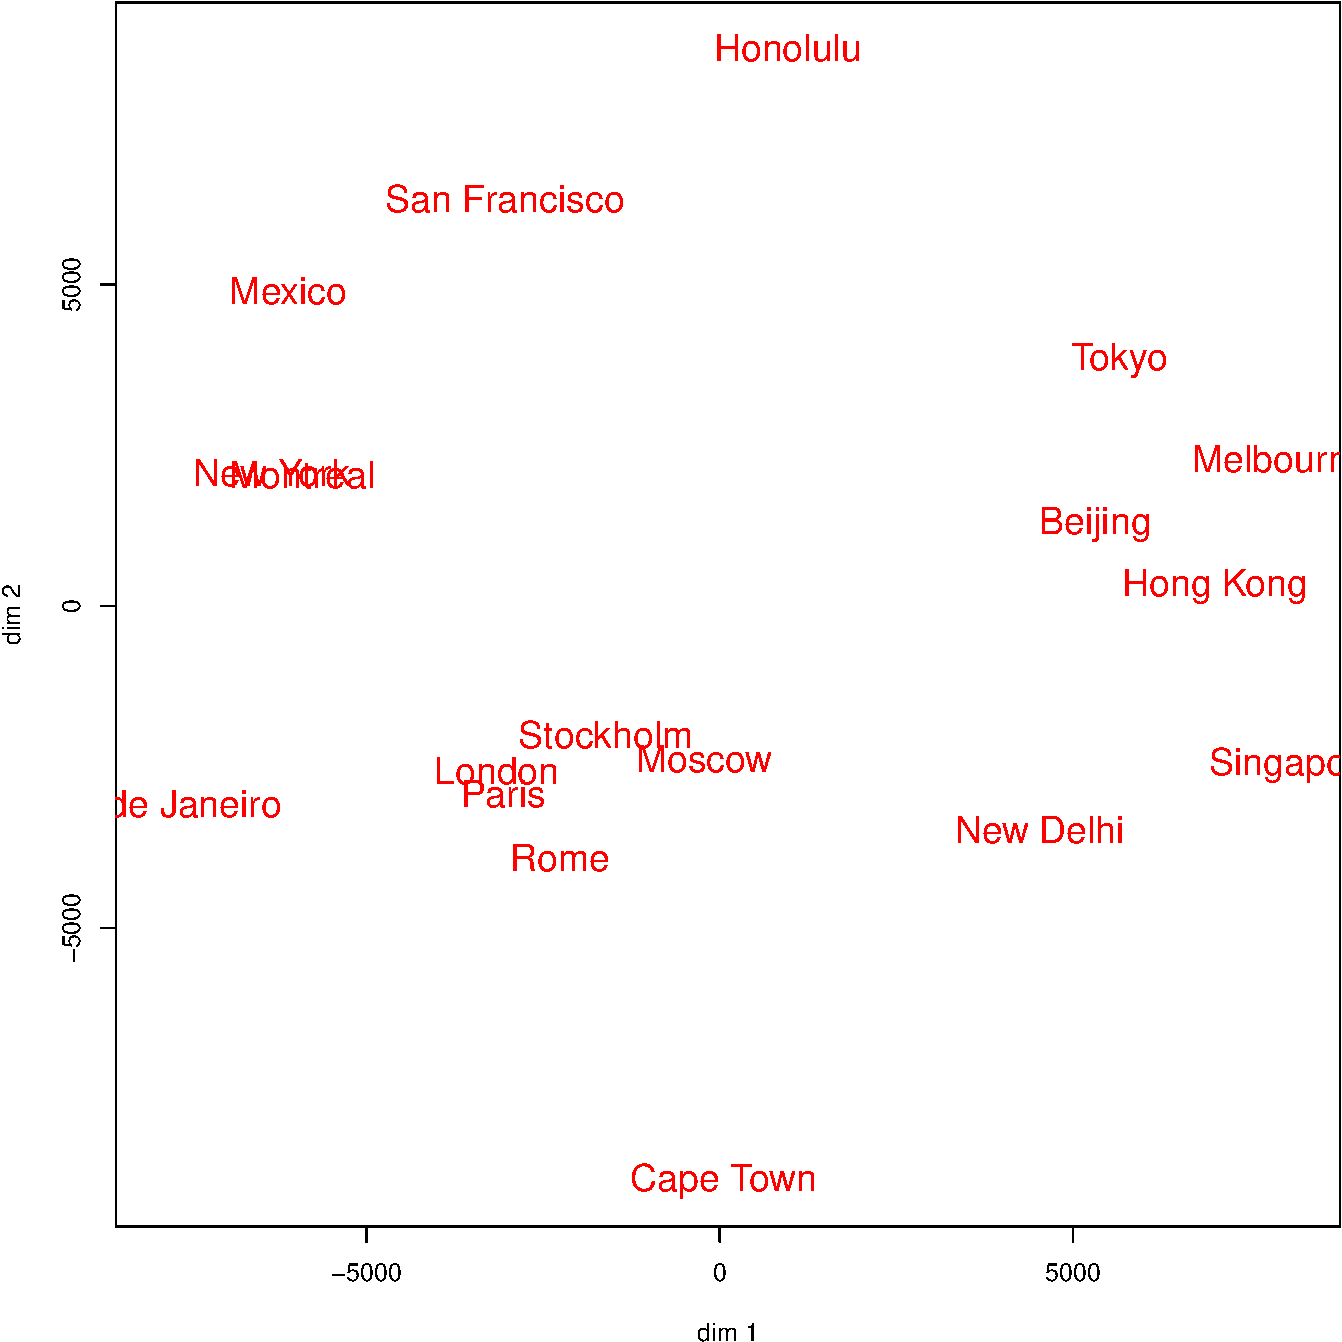
\includegraphics[keepaspectratio]{schoenemann_files/figure-pdf/acomplot-1.pdf}}

}

\caption{Airline Distances, Configuration Plot, Complete Data}

\end{figure}%

\begin{figure}[H]

{\centering \pandocbounded{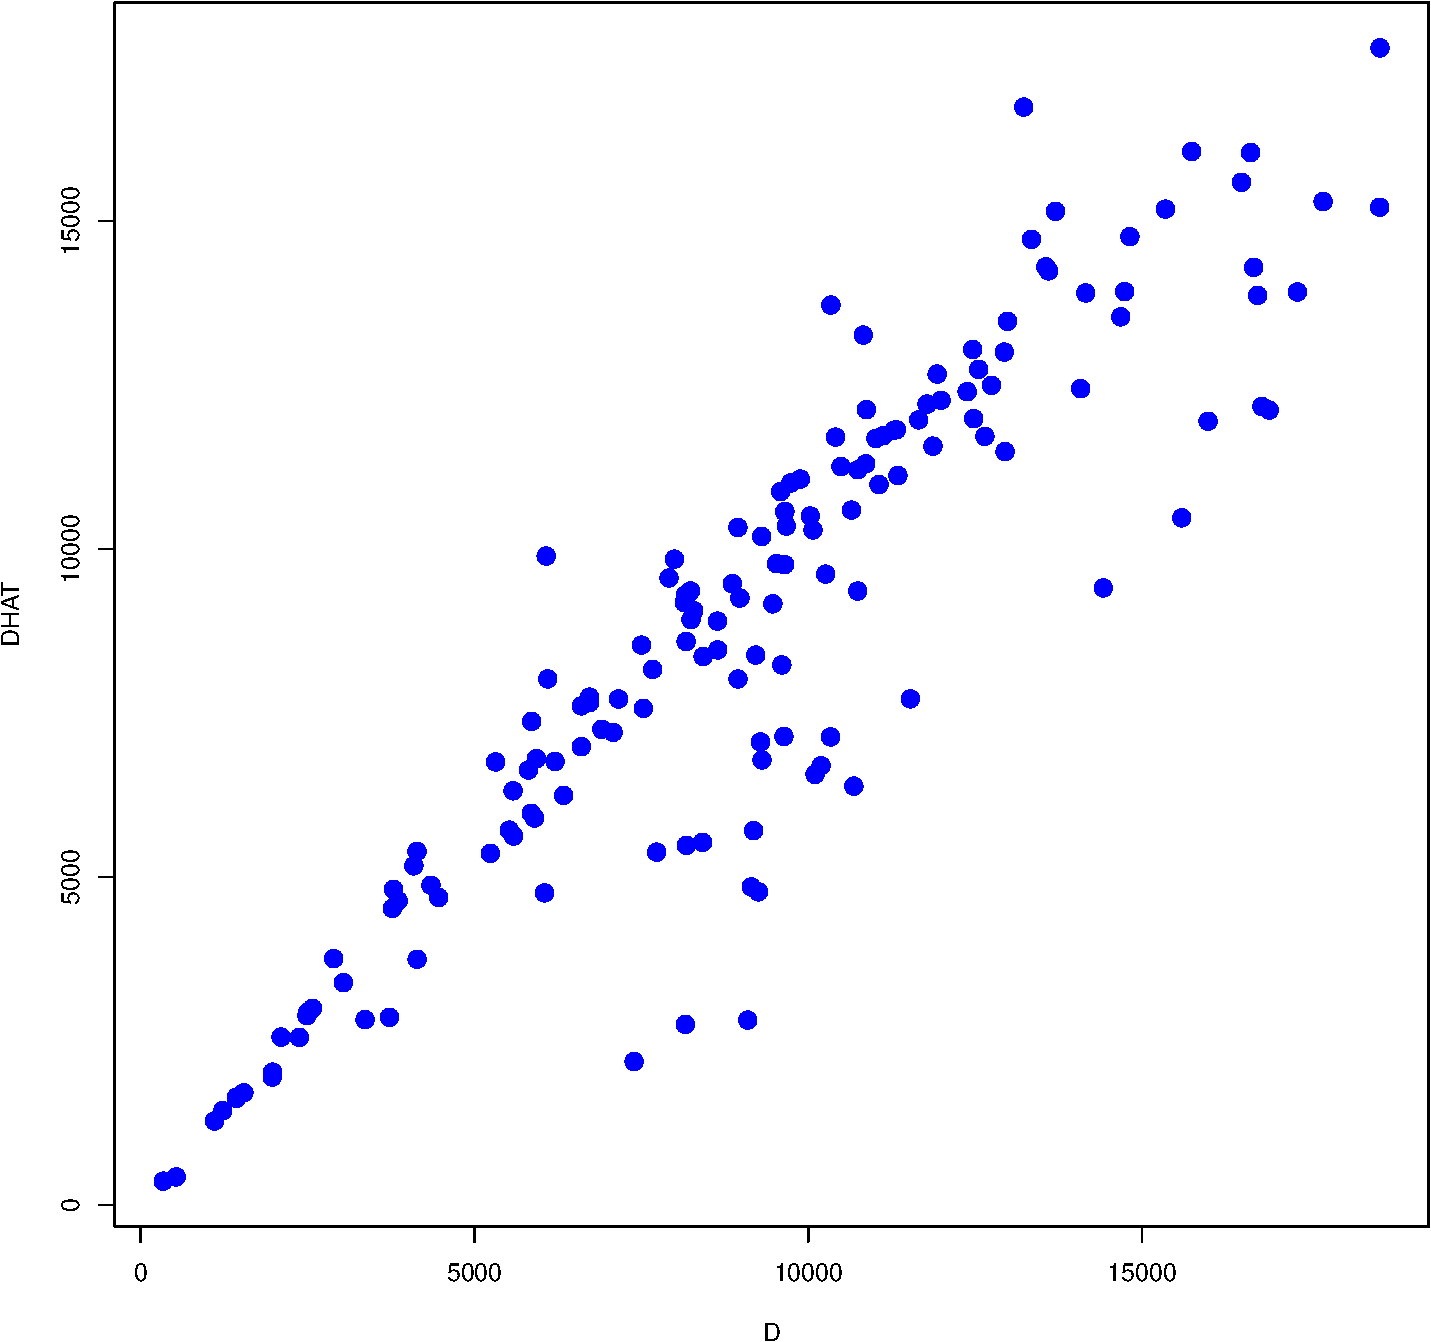
\includegraphics[keepaspectratio]{schoenemann_files/figure-pdf/acomplot2-1.pdf}}

}

\caption{Airline Distances, Dist-Dhat Plot, Complete Data}

\end{figure}%

We now create a \(9\times 9\) off-diagonal submatrix by using the
even-numbered cities as rows and the rest as columns. The transpose of
the submatrix is also analyzed. Although the two dimensions from the
complete solution are still there the plots have some distortions

\begin{figure}[H]

{\centering \pandocbounded{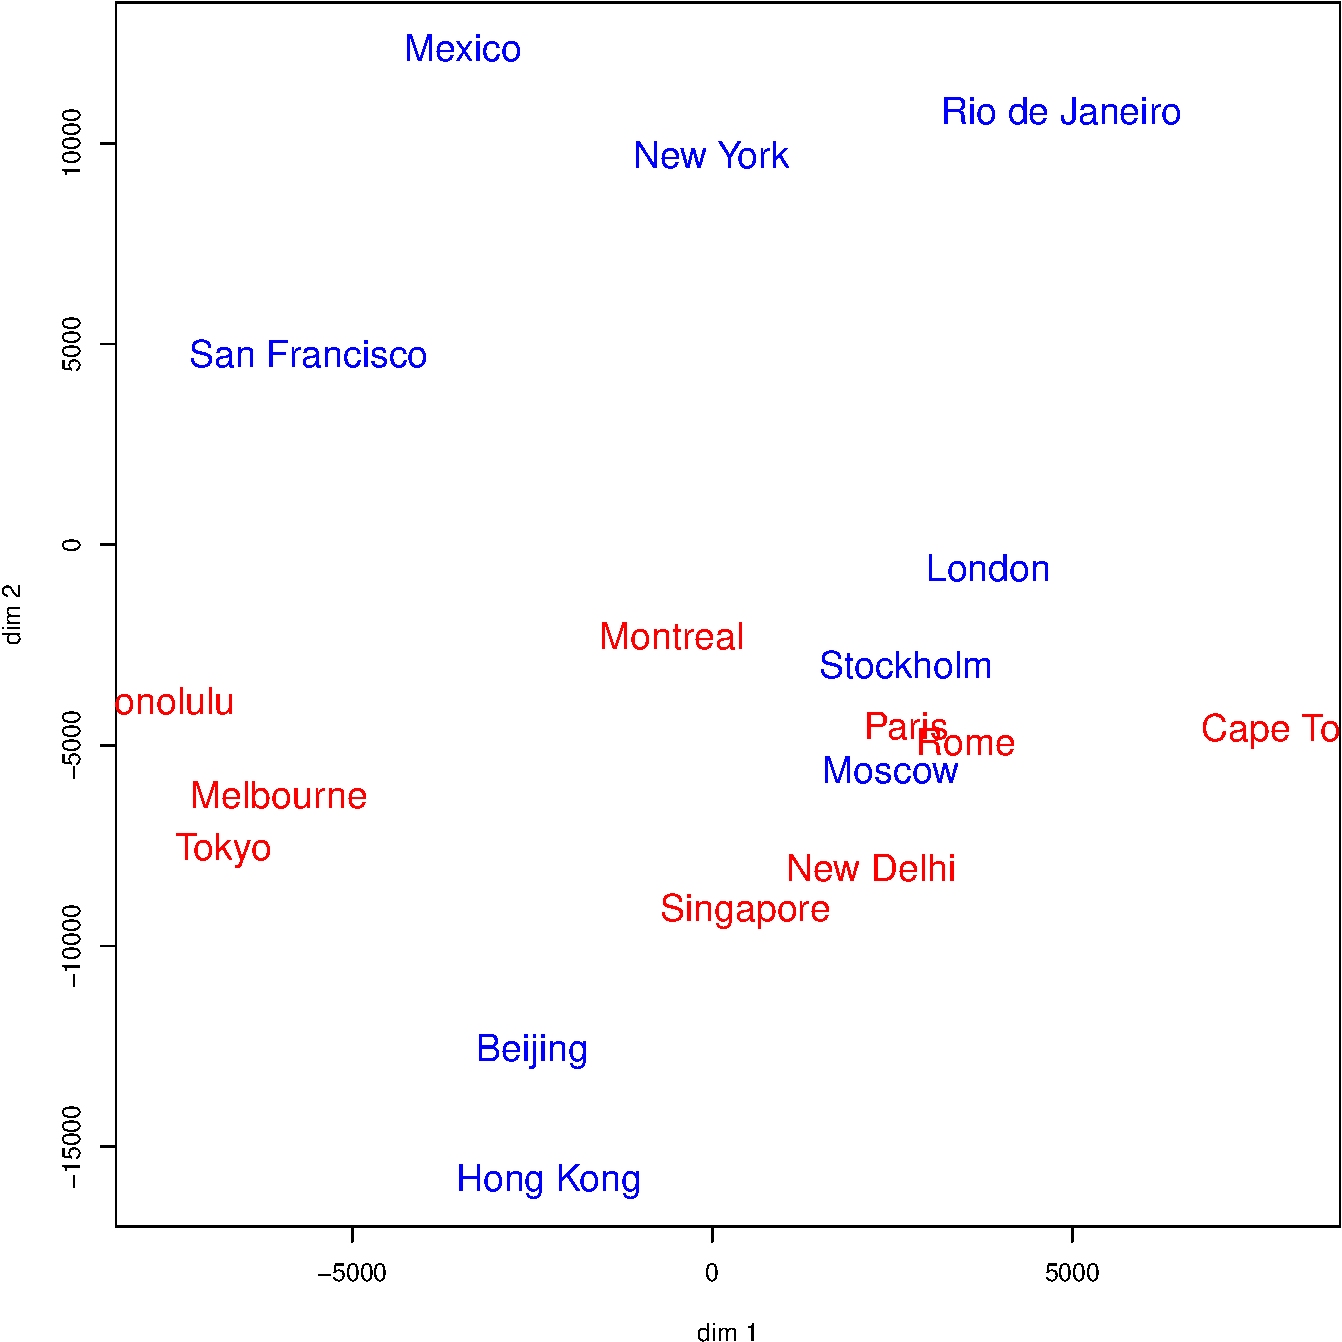
\includegraphics[keepaspectratio]{schoenemann_files/figure-pdf/airect1-1.pdf}}

}

\caption{Airline Distances, Configuration Plot, Off-diagonal Submatrix}

\end{figure}%

\begin{figure}[H]

{\centering \pandocbounded{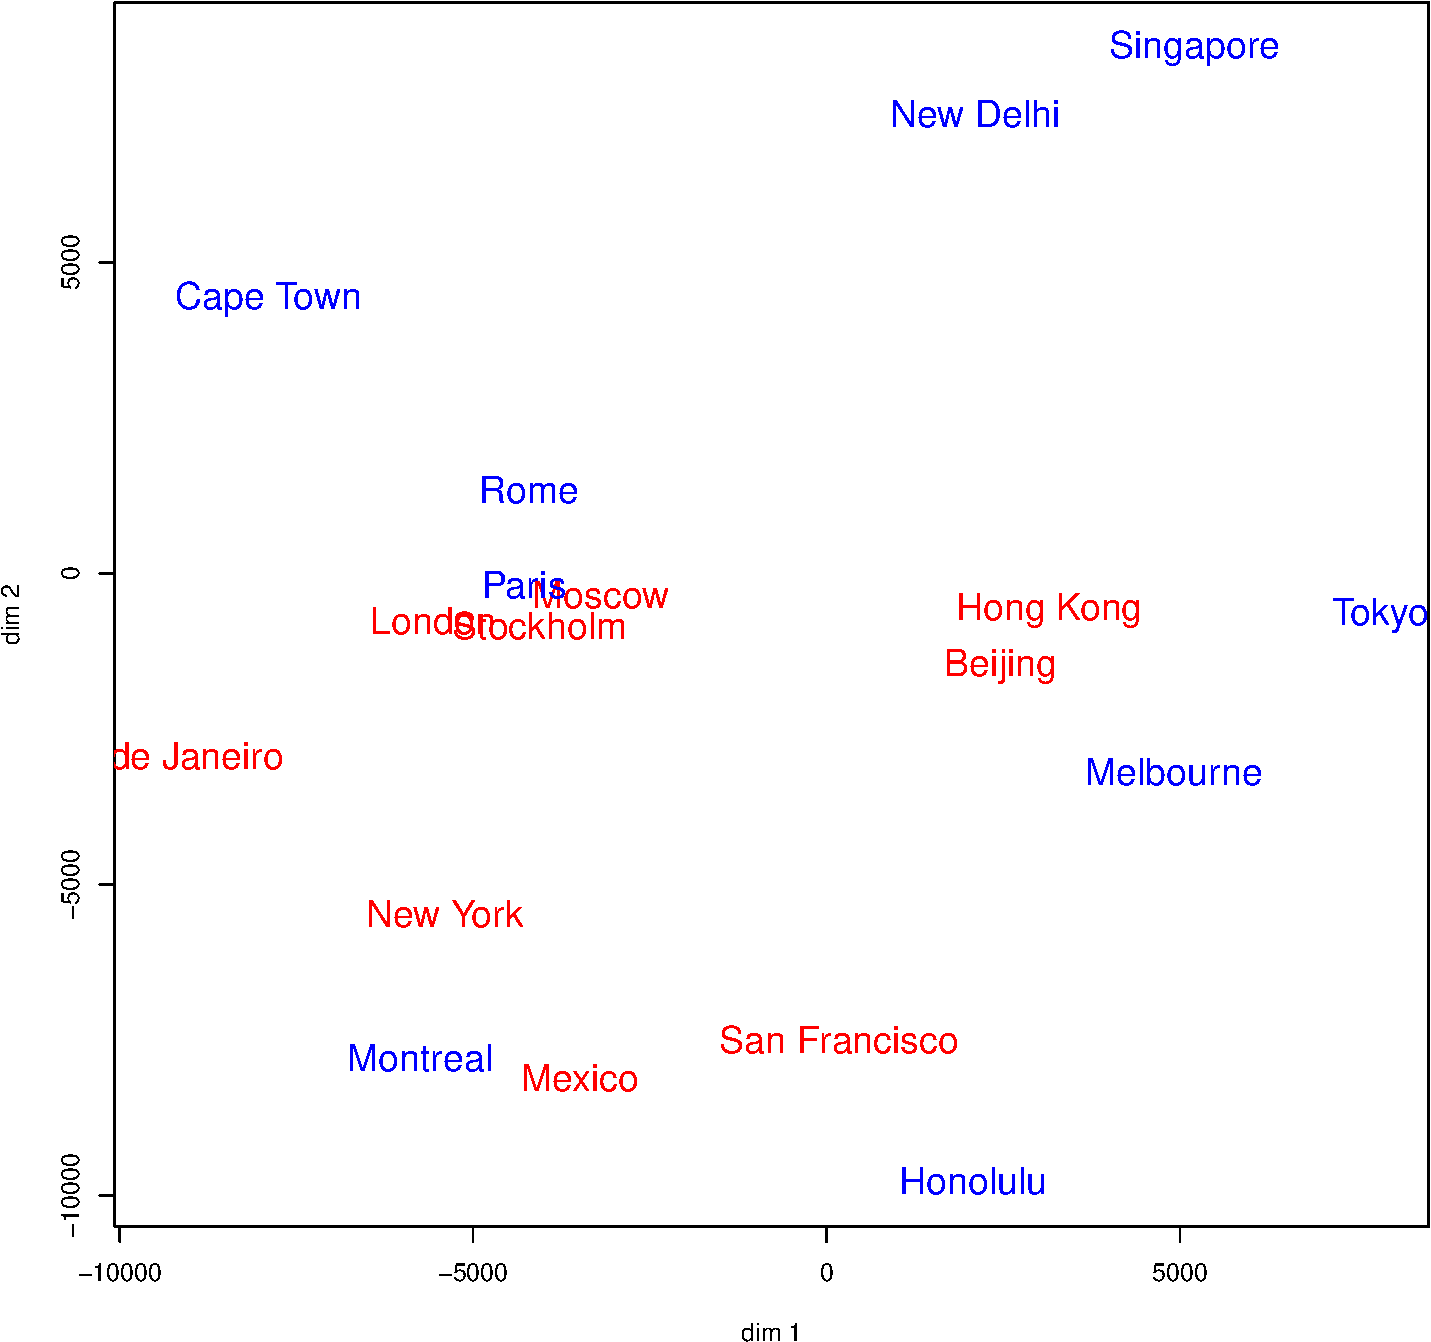
\includegraphics[keepaspectratio]{schoenemann_files/figure-pdf/airect2-1.pdf}}

}

\caption{Airline Distances, Configuration Plot, Off-diagonal Submatrix,
Transposed}

\end{figure}%

\subsection{Gold}\label{gold}

Our next example is the same as the one in Heiser and De Leeuw
(\citeproc{ref-heiser_deleeuw_A_79}{1979}). The data are taken from the
\emph{Power in the Classroom} study of Gold
(\citeproc{ref-gold_58}{1956}). Children in elementary school, divided
into eight groups, judge how important 17 characteristics of their
classmates are for their power in the classroom. Data are the times each
of properties were rated as ``very important'' by the eight age-sex
groups. The groups have three-digit codes in the joint configuration
plot. The first digit indicates the school grade (third vs higher), the
second the gender of the respondent, the third indicates the importance
of the property rated for males or females.

We first give the configuration plot and the Dist-Dhat plot. For the ''
f average'' analysis.

\begin{figure}[H]

{\centering \pandocbounded{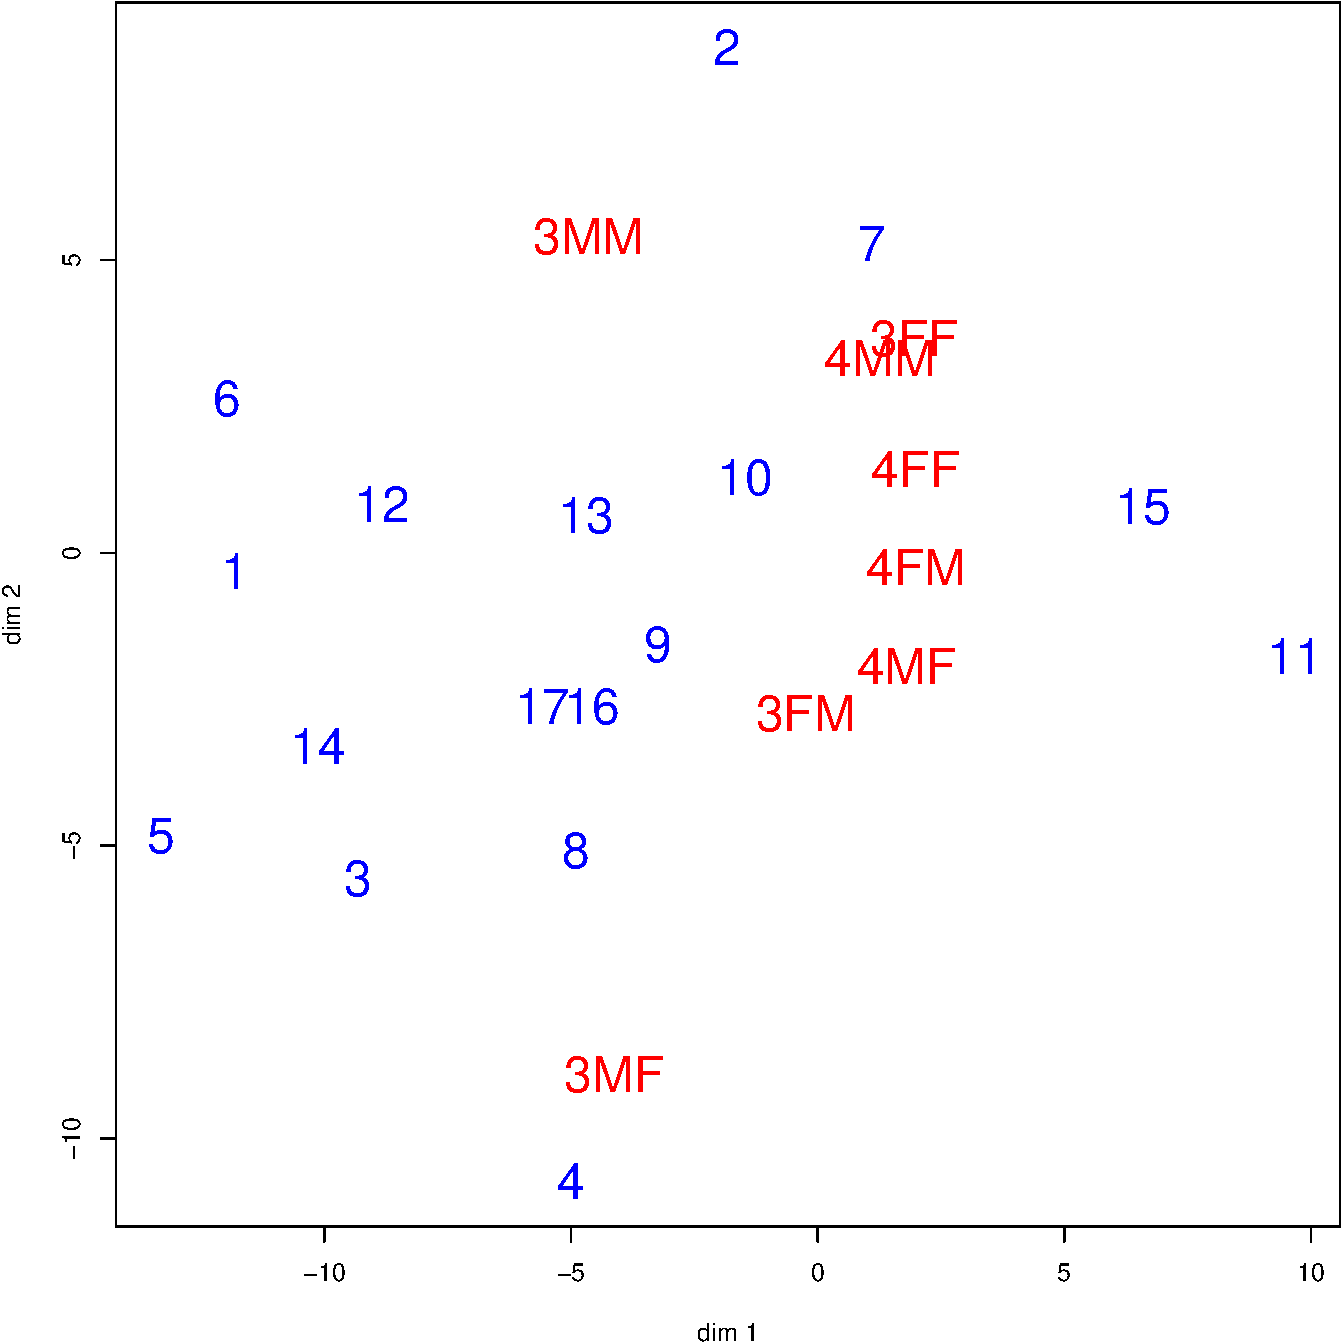
\includegraphics[keepaspectratio]{schoenemann_files/figure-pdf/jplot-1.pdf}}

}

\caption{Gold Data, Configuration Plot}

\end{figure}%

\begin{figure}[H]

{\centering \pandocbounded{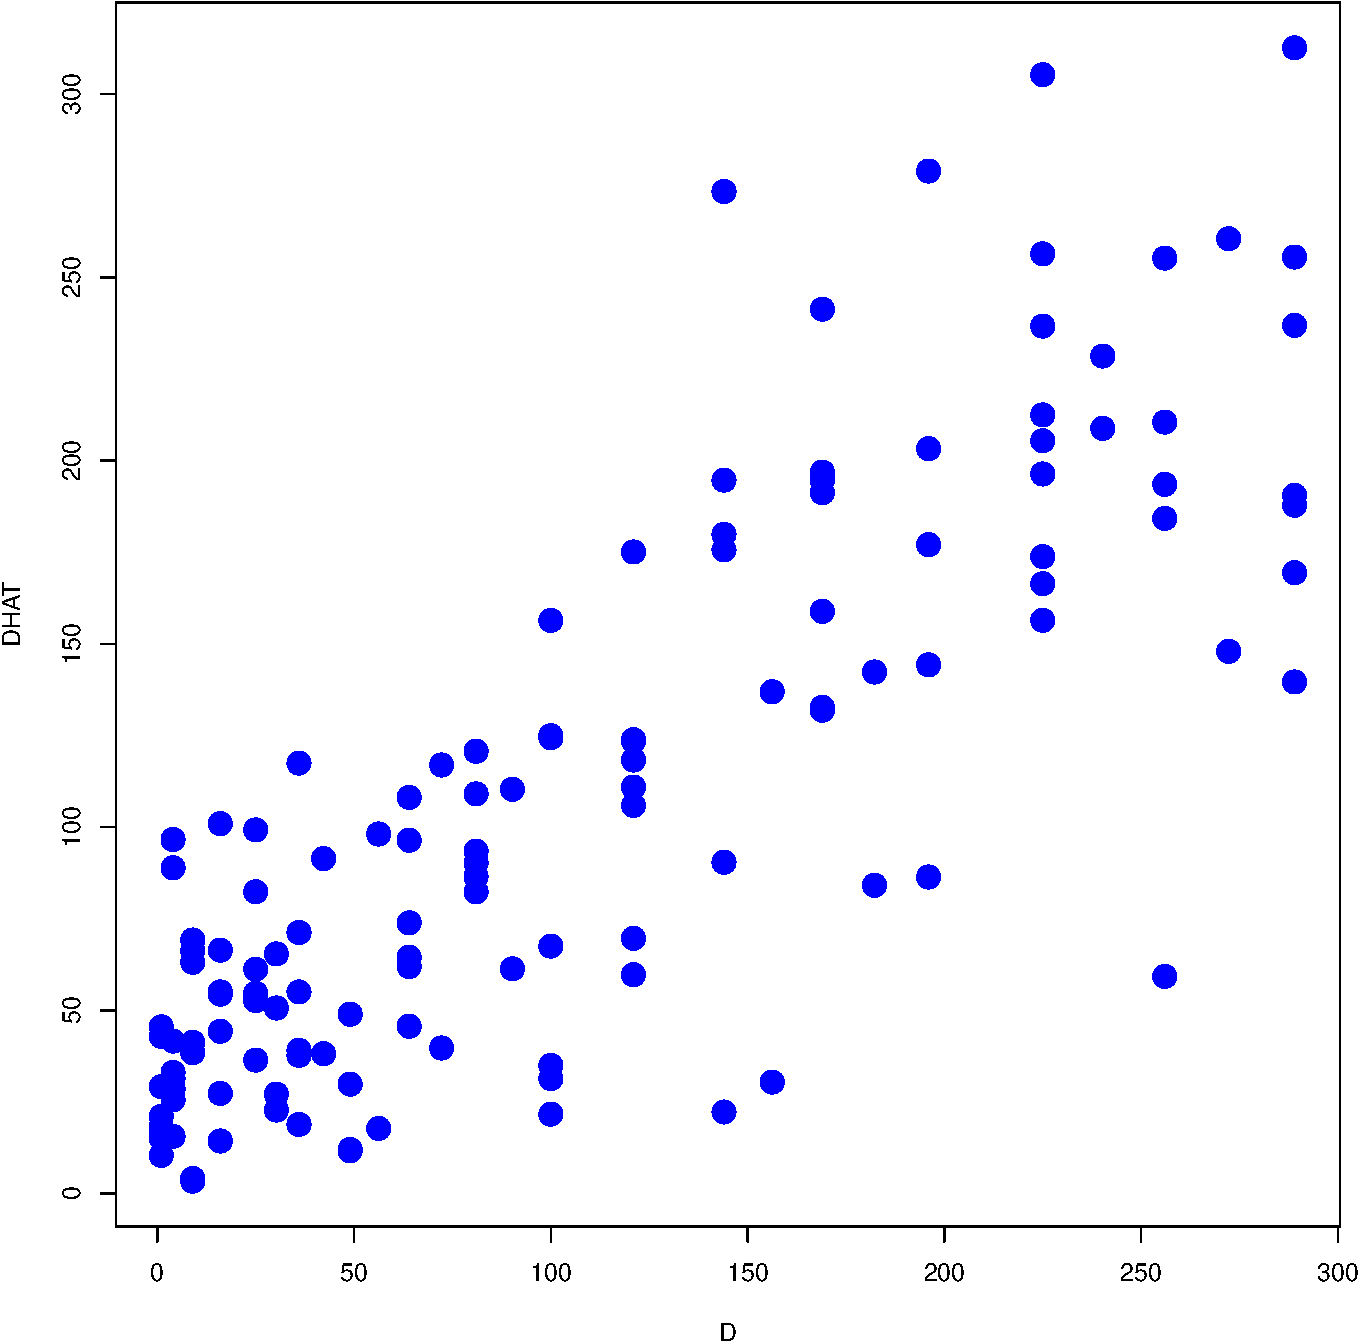
\includegraphics[keepaspectratio]{schoenemann_files/figure-pdf/dplot-1.pdf}}

}

\caption{Gold Data, Dist-Dhat Plot}

\end{figure}%

Next, we perform an analysis for each of the columns of \(F\)
separately, and we plot the solutions for the column scores \(Y\) in a
single plot (without matching them with rotation and translation). We
overlay the result with the result of the average analysis (in red).

\begin{figure}[H]

{\centering \pandocbounded{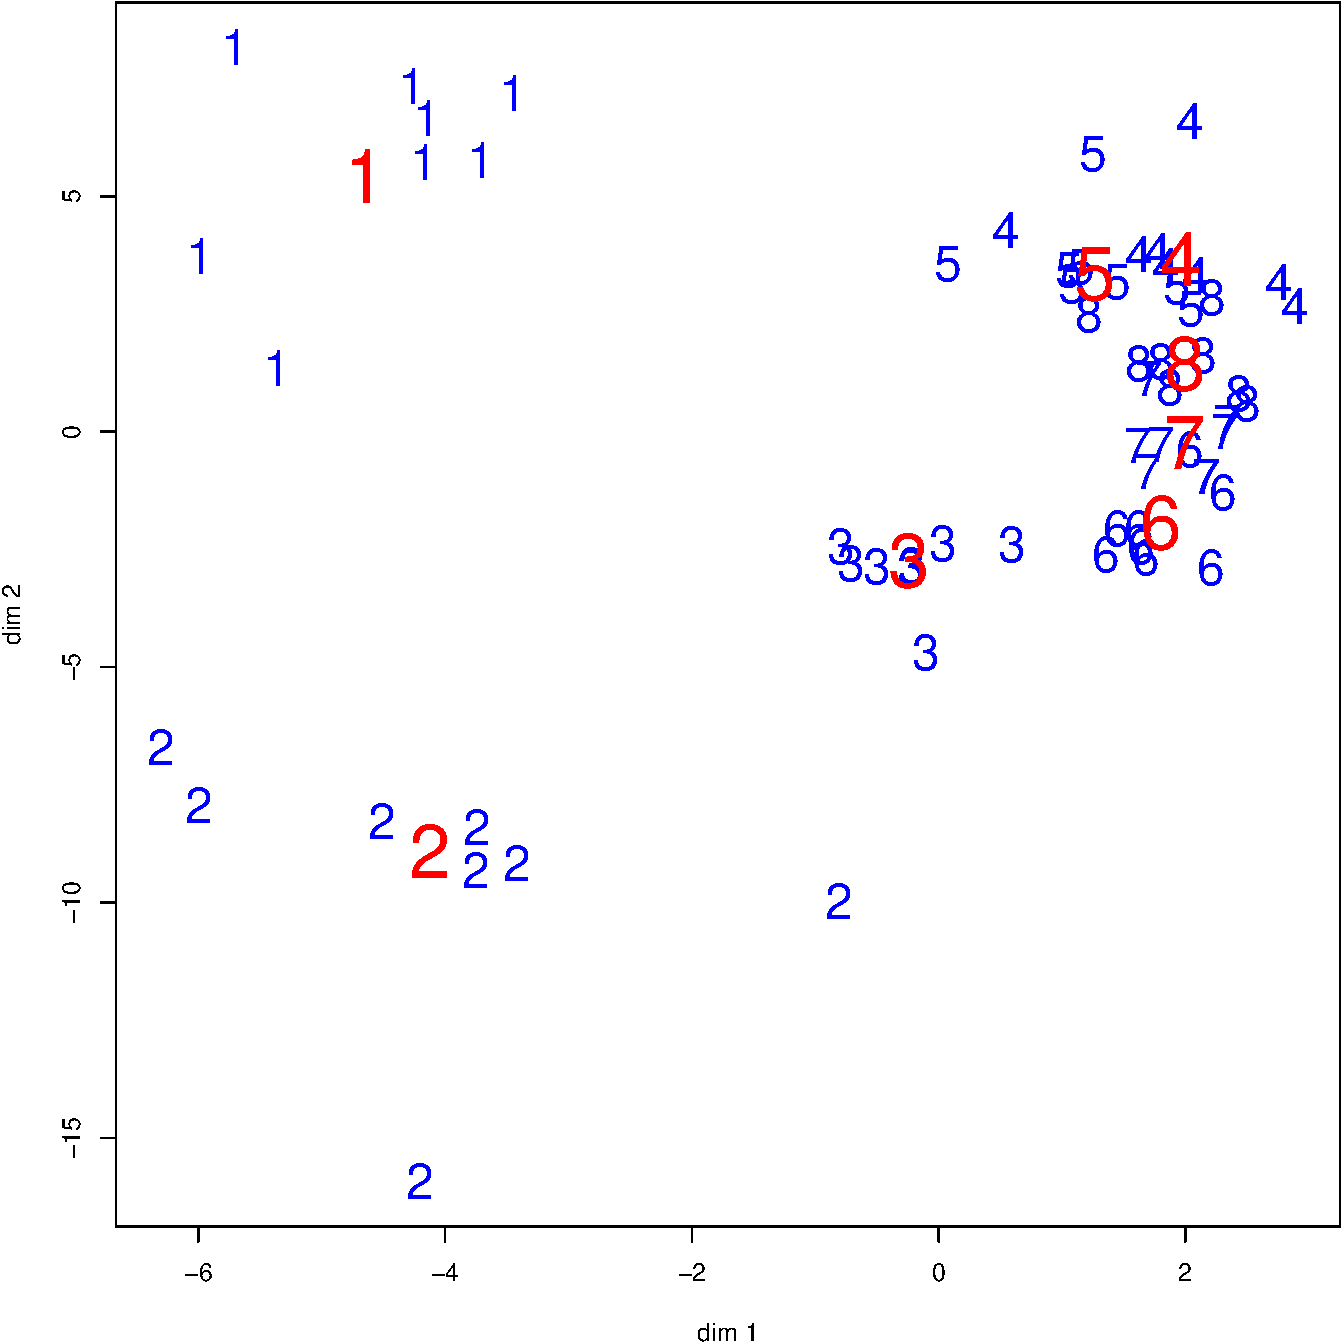
\includegraphics[keepaspectratio]{schoenemann_files/figure-pdf/yplot-1.pdf}}

}

\caption{Gold Data, Column Configuration from Eight Column and One
Average Analysis}

\end{figure}%

The solution seems to be quite stable over column-selection. It should
be noted that if we go to three dimensions, or if we transpose the
analysis, the matrix \(M\) is no longer positive definite.

\subsection{Roskam}\label{roskam}

In 1968 Roskam (\citeproc{ref-roskam_68}{1968}) asked 39 of the staff
members of the Psychology Laboratory at Nijmegen University to rank the
nine different departments in the laboratory as to the importance for
their work. The departments are

\begin{enumerate}
\def\labelenumi{\arabic{enumi}.}
\tightlist
\item
  Social Psychology
\item
  Educational and Developmental Psychology
\item
  Clinical Psychology
\item
  Mathematical Psychology and Statistics
\item
  Experimental Psychology
\item
  Cultural Psychology and Psychology of Religion
\item
  Industrial Psychology
\item
  Test Construction and Validation
\item
  Physiological and Animal Psychology
\end{enumerate}

Thus the data are 39 rank orders. It seems rather procrustean to
approximate discrete rank numbers by continuous distances. Moreover the
data are conditional, which means that a rank equal to five for staff
member A may not have the same ``meaning'' as a five for staff member B.
Nevertheless we use these data for our example, since it is after all an
off-diagonal rectangular matrix with positive numbers.

All rows of \(D\) add up to 45, so if we were to choose row-means for
\(f\) they would be exactly zero. If we use all of the 9 rows of \(F\)
in turn, then for six of them we find that \(M\) is indefinite. The
configurations for rows 1, 2, and 7 are plotted. There is clearly a
worse fit, and much less stability, than in the Gold example. The most
important difference between the three analyses is the relative size of
the row and column configurations.

\begin{figure}[H]

{\centering \pandocbounded{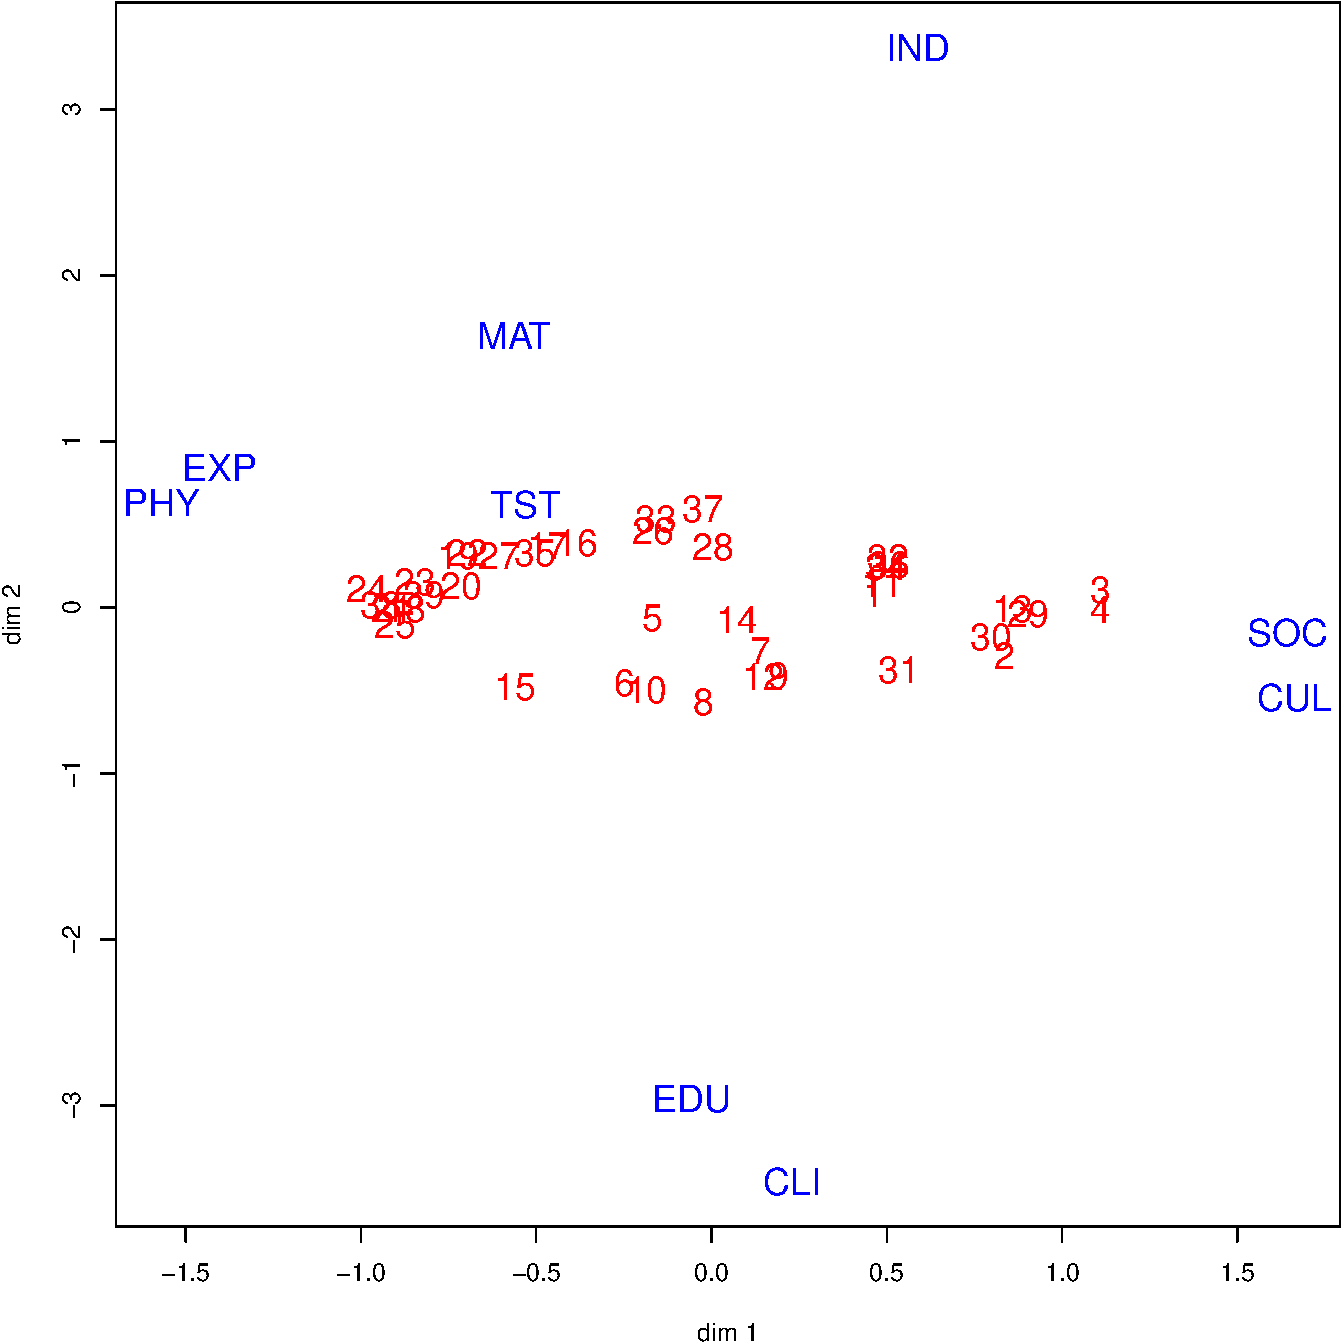
\includegraphics[keepaspectratio]{schoenemann_files/figure-pdf/rosplot1-1.pdf}}

}

\caption{Roskam Data, Configuration Plot from Column 1}

\end{figure}%

\begin{figure}[H]

{\centering \pandocbounded{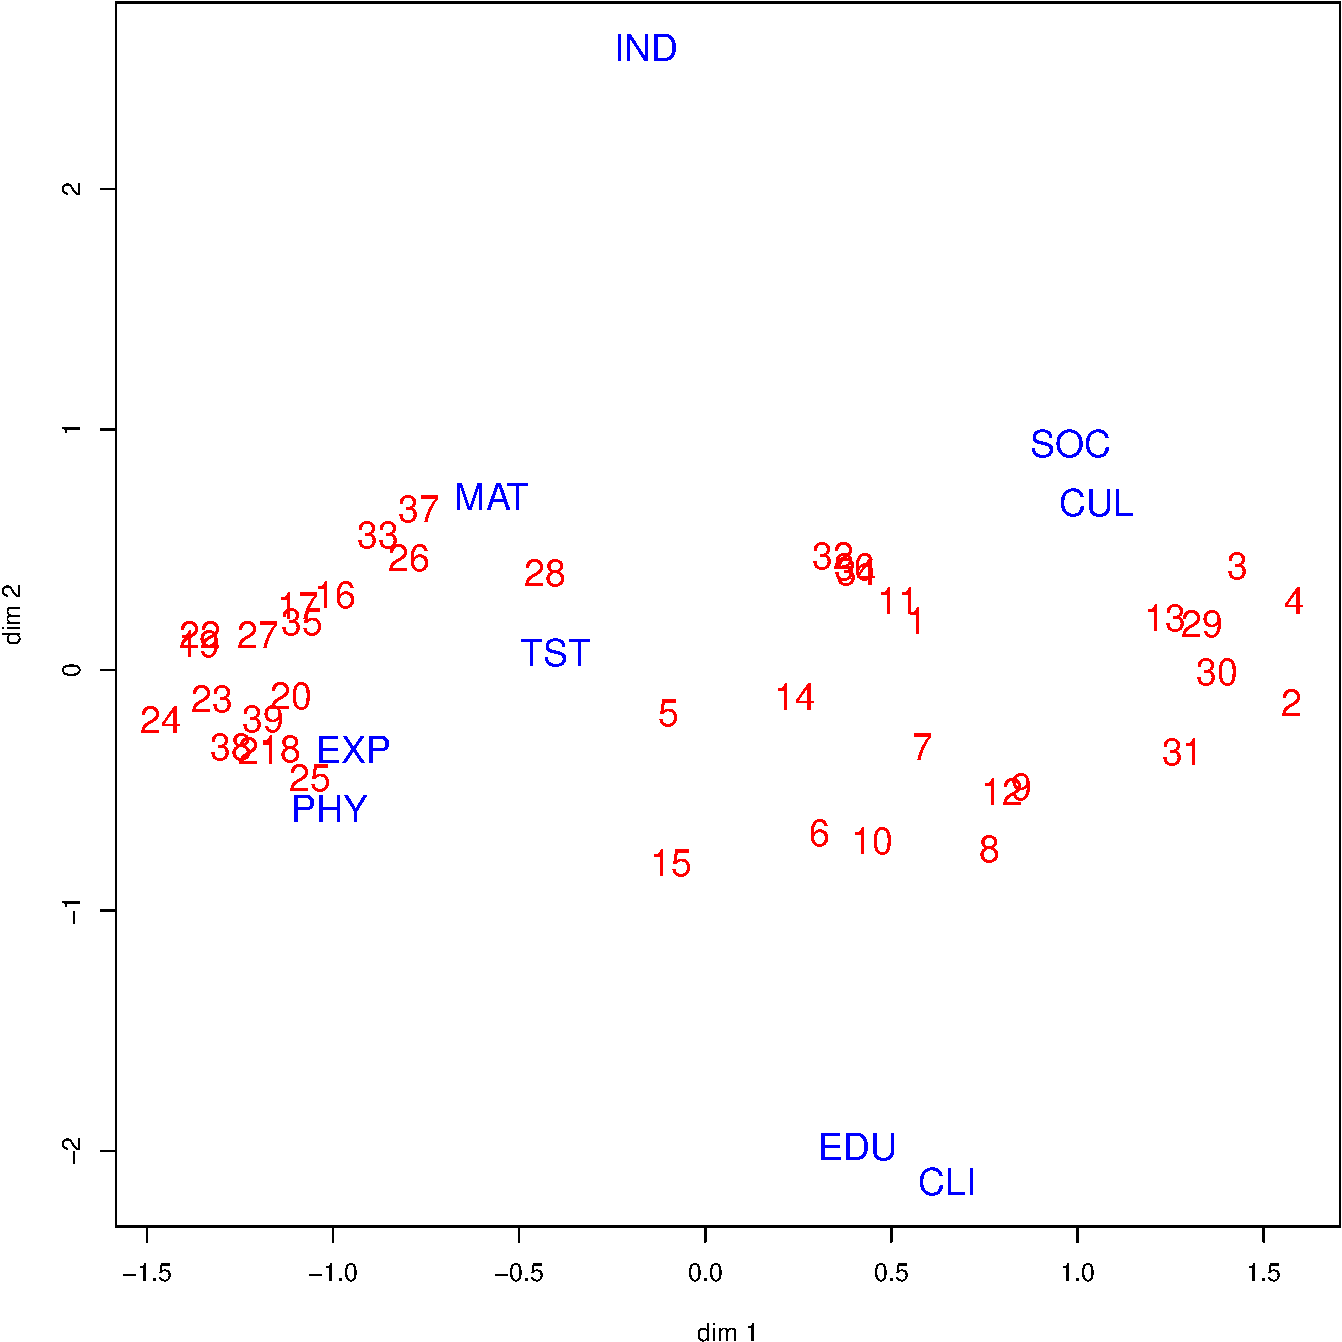
\includegraphics[keepaspectratio]{schoenemann_files/figure-pdf/rosplot2-1.pdf}}

}

\caption{Roskam Data, Configuration Plot from Column 2}

\end{figure}%

\begin{figure}[H]

{\centering \pandocbounded{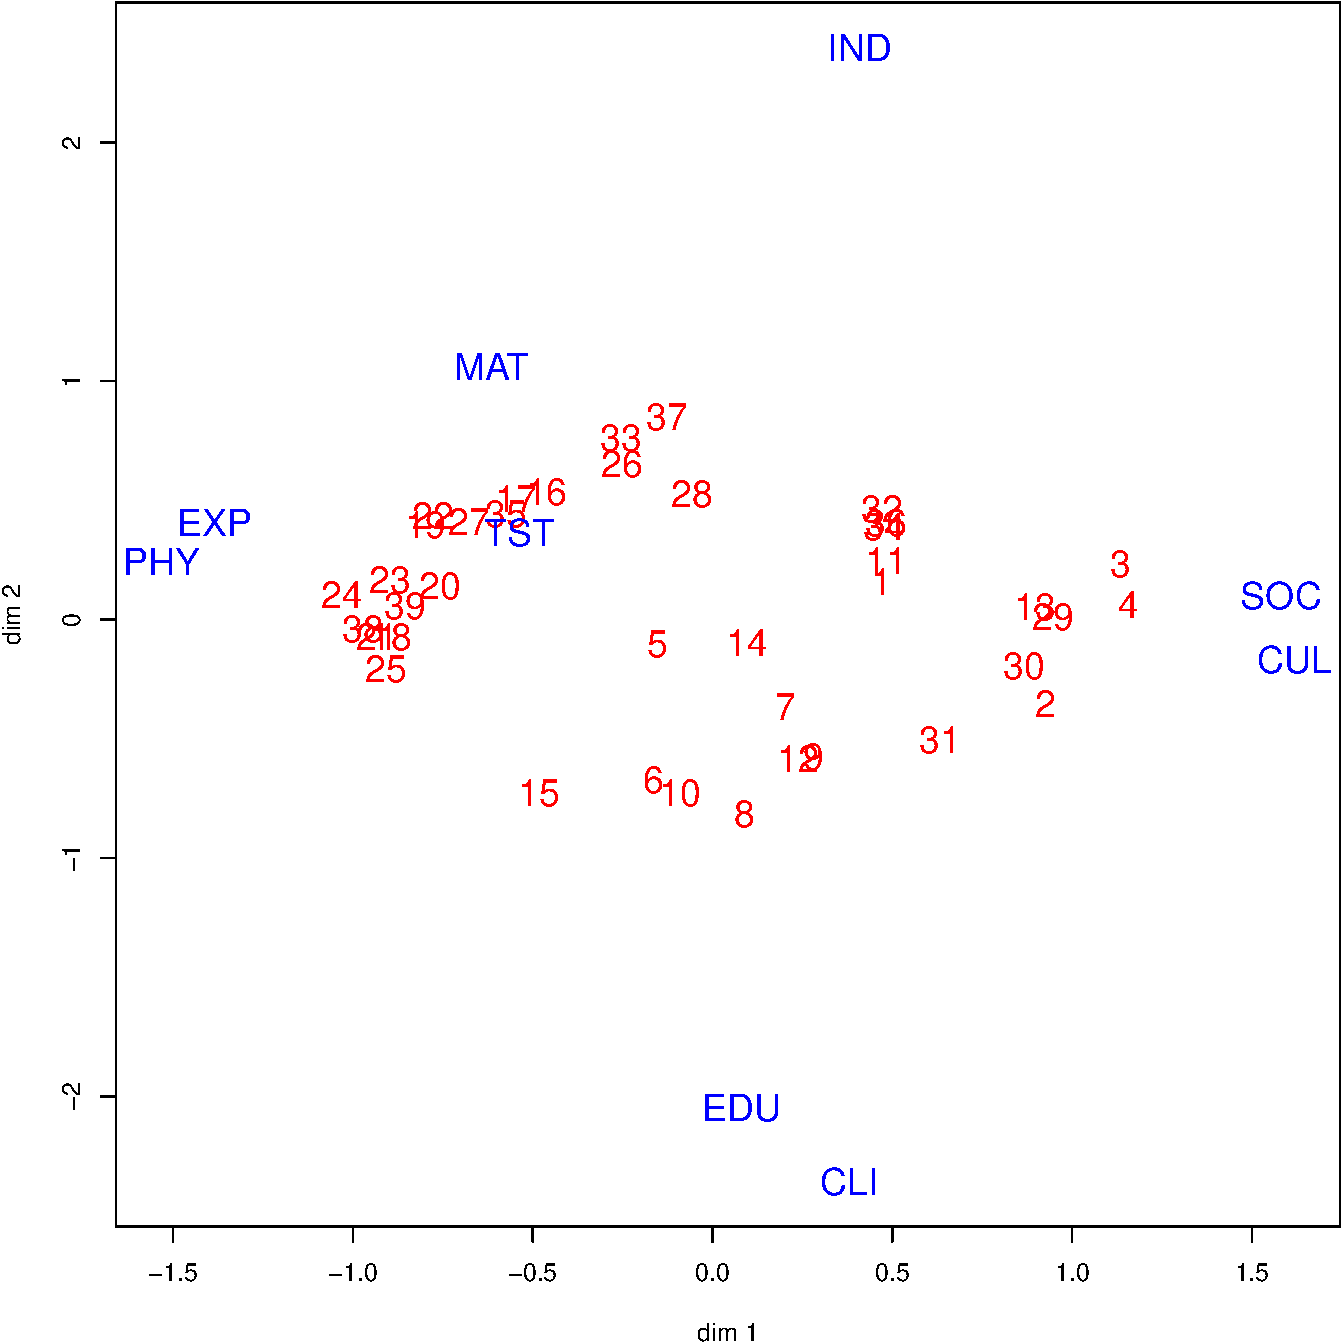
\includegraphics[keepaspectratio]{schoenemann_files/figure-pdf/rosplot3-1.pdf}}

}

\caption{Roskam Data, Configuration Plot from Column 7}

\end{figure}%

The D-Dhat plot for the column seven solution shows the poor fit (due
mostly to fitting distances to rank numbers). The red line shows the
average Dhat value for each distance category, indicating at least some
degree of monotonicity.

\begin{figure}[H]

{\centering \pandocbounded{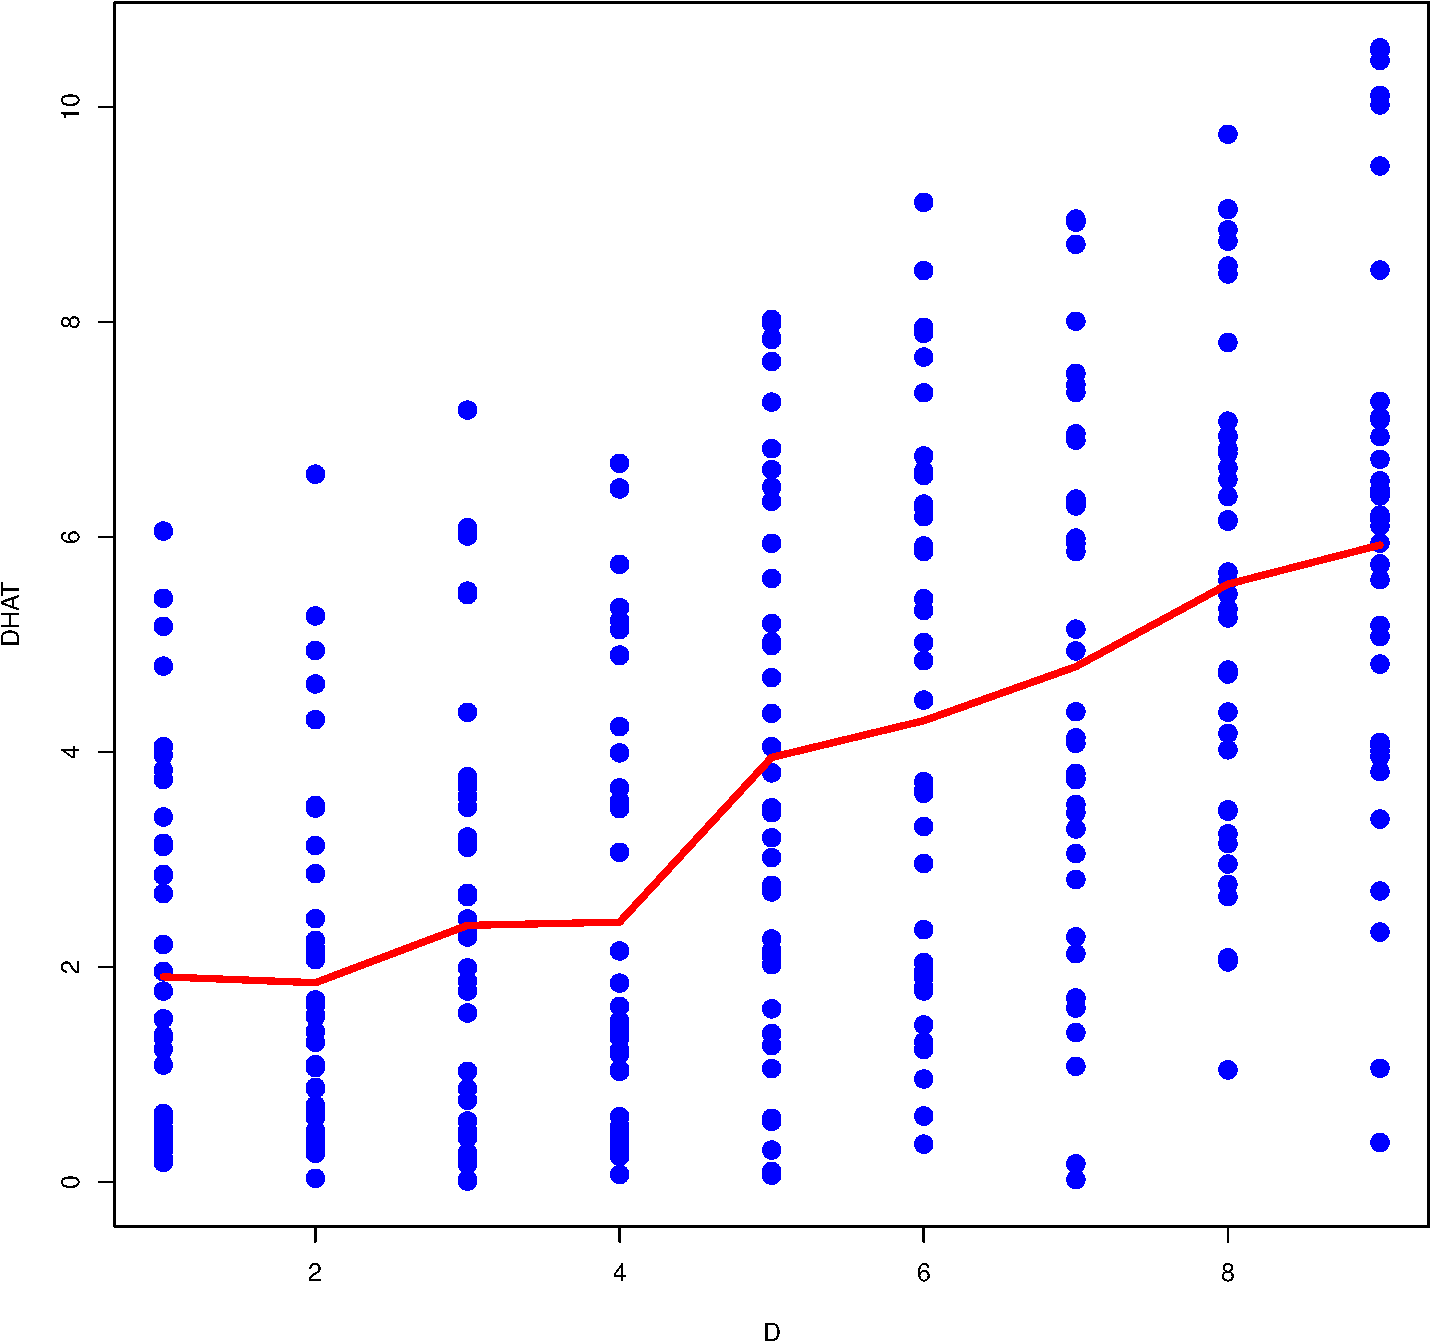
\includegraphics[keepaspectratio]{schoenemann_files/figure-pdf/rosdd-1.pdf}}

}

\caption{Roskam Data, D-DHAT plot, Column 7 Solution}

\end{figure}%

\sectionbreak

\section{Software}\label{software}

The function schoenemann() in the file schoenemann.R implements the
``row-oriented'' solution to perfect or imperfect data. We choose a
value of \(p\), with \(p=2\) the default. The singular value
decomposition is used to approximate \(D\) by a matrix of rank \(p\). We
then compute \(\tilde F\). If the parameter fsel is zero, \(f\) are the
row-averages of \(\tilde F\). If fsel is equal to \(j\) then \(f\) is
column \(j\) of \(\tilde F\). The R function lm.fit() is used to find
the least squares solution of the linear system \ldots, and the program
gives a warning if the estimated rank of \(K\) is less than its number
of columns \(\frac12 p(p+3)\). From the solution we reconstruct \(M\),
and again a warning is issued if \(M\) is not positive definite. The R
function eigen() uses \(M=L\Lambda L'\) to test for positive
definiteness. If some eigenvalues are negative then we replace them by
their absolute values. There is not real convincing justification for
this, except the lame excuse that if \(M\), which is of order \(p\),
only has small negative eigenvalues then we only make a small
unjustified adjustment. The function schoenemann() does return
\(\tilde F\), \(K\), and \(M\) so we can do some post-hoc analyses to
see where things went wrong. In addition solutions \(X\) and \(Y\), with
corresponding \(D(X,Y)\) are returned, as well as the input matrix
\(D\).

\sectionbreak

\section*{References}\label{references}
\addcontentsline{toc}{section}{References}

\phantomsection\label{refs}
\begin{CSLReferences}{1}{0}
\bibitem[\citeproctext]{ref-borg_groenen_05}
Borg, Ingwer, and Patrick J. F. Groenen. 2005. \emph{Modern
Multidimensional Scaling}. Second Edition. Springer.

\bibitem[\citeproctext]{ref-gold_58}
Gold, Martin. 1956. {``Power in the Classroom.''} \emph{Sociometry} 21
(1): 50--60.

\bibitem[\citeproctext]{ref-gower_66}
Gower, John C. 1966. {``{Some Distance Properties of Latent Root and
Vector Methods Used in Multivariate Analysis}.''} \emph{Biometrika} 53:
325--38.

\bibitem[\citeproctext]{ref-heiser_deleeuw_A_79}
Heiser, Willem J., and Jan De Leeuw. 1979. {``Metric Multidimensional
Unfolding.''} \emph{{Methoden En Data Nieuwsbrief SWS/VVS}} 4: 26--50.
\url{https://jansweb.netlify.app/publication/heiser-deleeuw-a-79/heiser-deleeuw-a-79.pdf}.

\bibitem[\citeproctext]{ref-roskam_68}
Roskam, E. E. 1968. {``{Metric Analysis of Ordinal Data in
Psychology}.''} PhD thesis, University of Leiden.

\bibitem[\citeproctext]{ref-schoenberg_35}
Schoenberg, Isaac J. 1935. {``{Remarks to Maurice Frechet's article: Sur
la Definition Axiomatique d'une Classe d'Espaces Vectoriels Distancies
Applicables Vectoriellement sur l'Espace de Hllbert}.''} \emph{Annals of
Mathematics} 36: 724--32.

\bibitem[\citeproctext]{ref-schoenemann_70}
Schönemann, Peter H. 1970. {``{On Metric Multidimensional Unfolding}.''}
\emph{Psychometrika} 35 (3): 349--66.

\bibitem[\citeproctext]{ref-torgerson_58}
Torgerson, Warren S. 1958. \emph{{Theory and Methods of Scaling}}. New
York: Wiley.

\bibitem[\citeproctext]{ref-young_householder_38}
Young, Gale, and Alston S. Householder. 1938. {``{Discussion of a Set of
Points in Terms of Their Mutual Distances}.''} \emph{Psychometrika} 3
(19-22).

\end{CSLReferences}




\end{document}
